\documentclass[a4paper]{scrreprt}

\usepackage[T1]{fontenc}
\usepackage[utf8]{inputenc}
\pdfoptionpdfminorversion 7
\usepackage{graphicx}
\usepackage{amsmath}
\usepackage{svg}
\usepackage{listings}
%\usepackage{showframe}
\usepackage{fullpage}
\usepackage[colorlinks=true]{hyperref}
\usepackage{tabu}
\usepackage{float}
\usepackage{afterpage}
\usepackage{pdflscape}
\usepackage{pdfpages}
\usepackage[abs]{overpic}
\usepackage{nth}
\usepackage{siunitx}

\renewcommand{\thefootnote}{\fnsymbol{footnote}}

\graphicspath{{./fig/}}

\lstdefinelanguage[ARM]{Assembly}     % add a "x64" dialect of Assemblers
   [x86masm]{Assembler} % based on the "x86masm" dialect
   % with these extra keywords:
   {
   morekeywords={ADDS, ANDS, B, LDR, MOV, ORRS},
    morekeywords=[2]{.align,.cpu,.thumb,.syntax,.word},%
    alsoletter={.,0,1,2,3,4,5,6,7,8,9},%
    alsodigit={?},%
    sensitive=false,%
    morestring=[b]",%
    morecomment=[s]{/*}{*/},%
    morecomment=[l]@,%
    morecomment=[l]//,%
   }[keywords,comments,strings]
\lstset{language=[ARM]Assembly}

\lstdefinestyle{BashStyle}{
  language=bash,
  basicstyle=\small\ttfamily,
  %numbers=left,
  %numberstyle=\tiny,
  %numbersep=3pt,
  frame=tb,
  columns=fullflexible,
  %backgroundcolor=\color{yellow},
  linewidth=0.9\linewidth,
  xleftmargin=0.1\linewidth
}

\title{\vspace*{60mm}Introduction to Microcontrollers Notes}
\author{James Gowans}

\begin{document}
  \maketitle

  \vspace{\fill}
\section*{Licence}
This work is licensed under the Creative Commons Attribution-ShareAlike 3.0 Unported License. To view a copy of this license, visit http://creativecommons.org/licenses/by-sa/3.0/ or send a letter to Creative Commons, 444 Castro Street, Suite 900, Mountain View, California, 94041, USA.


\newpage
\tableofcontents
\newpage
%\chapter{A History of Processing}

\section{Babbage Difference Engine{

\section{Turing Machine}
Universal Turing machine?

\section{Jacquard loom}

\section{UNIVAC}

\section{Manchester Small-Scale Experimental Machine}
Stored program computer

\section{Cray-1}

\section{Cray-2}

\section{Commodore 64}

\section{Intel 4004}

\section{Intel 8008}

\section{Intel 8080}

\section{ARM}
In 1971 the dawn of a new era began. Intel had just announced that they had developed ``a programmable computer on a chip.'' The chip, known as the 4004 was the first general purpose microprocessor on one silicon chip, and contained around 2300 transistors. In order to produce this chip, the layout of the transistors was hand-drawn using coloured pencils at 500 times scale. The CPU had the ability to transfer 4 bits per clock cycle, had a 12-bit address space and an 8-bit instruction. In total, it has 16 instructions which it could execute. It was used in a calculator which had an optional square root function. The calculator run around 100K instructions per second, had 1 KB of ROM and 80 bytes of RAM. 

The next year, in 1972 Intel released the 8008, an 8-bit microprocessor. The 8008 had a 14 bit address space. The first use for the 8008 was a programmable scientific calculator. In 1973 the 8008 was used as the CPU for a French desktop computer. Some consider this to be the first desktop computer. The 8008 evolved into the 8080. 

While desktop computers do take a large share of the microprocessor market, many times more microprocessors go into microcontrollers for the purpose of embedded control applications. In 1996, 25 years after the advent of the first microprocessor, 70\% of all semiconductors are used for microcontroller-based circuits. 

A processor with IO an memory is a microcontroller. In 1995, 50\% of microcontrollers manufacturered were 4-bit. 

\chapter{System Overview}

\begin{figure}[t]
  \centering
  \includegraphics[width=\textwidth]{./fig/programmers_model_v0.pdf}
  \caption{The most simplified view of the internals of the STM32F051}
  \label{fig:prog_mod_v0}
\end{figure}

\section{What is a Microcontroller?}
The microcontroller can be understood by comparing it to something you are already very familiar with: the computer. Both a microcontroller and a computer can be modeled as a black box which takes in data and instructions, performs processing, and provides output.
In order to do this, a micro has some of the same internals as a computer, shown graphically in \autoref{fig:prog_mod_v0} and discussed now:
\begin{itemize}
  \item CPU: The section of the microcontroller which does the processing. It executes instructions which allows it to do arithmetic and logic operations, amongst other forms of operations.
  \item  Volatile memory (RAM:) This is general purpose memory. It can be used for storing whatever you want to store in it. Typically it stores variables which are created or changed during the course of execution of a program.
  \item Non-volatile memory (Flash): This non-volatile memory is used to store any date which must not be lost when the power to the micro is removed. Typically this would include the program code and any constants or initial values of data.
  \item Ports: Interfaces for data to move in and out of the micro. This allow it to communicate with the outside world. 
\end{itemize} 
These resources are typically orders of magnitude smaller or a micro than on a conventional computer. A micro makes up for this lack of resources with a small size, low power and low cost. A comparison of the characteristics can be seen in \autoref{table:specs_comp}.
A computer is typically defined as a multi-purpose, flexible unit able to do computation. A microcontroller on the other hand typically is hard-coded to do one specific job.\\

\begin{table}
\begin{tabu}{ >{\textbf}c | c  c  c  c  c  c }
  & \textbf{CPU} & \textbf{RAM} & \textbf{Non-volatile} & \textbf{Power} & \textbf{Size/Mass} & \textbf{Cost} \\
  \hline
  \textbf{Computer} & Dual, 3 GHz & 4 GiB & 500 GB & 100 W & Large & R 3000 \\
  \textbf{Micro} & 48 MHz & 8 KiB & 32 KiB & 50 mW & Small & R 15 \\
\end{tabu}
\caption{Comparison of specs of entry level computer to STM32F051C6.}
\label{table:specs_comp}
\end{table}

The terms micro\textit{controller} and micro\textit{processor} are different and should not be used interchangeably. A micro\textit{processor} is a chip which is able to perform computation, but requires external memory and peripherals to function. A micro\textit{controller} has the memory and peripherals built into it, allowing it to be fully independent. Furthermore, the interface in and out of a microprocessor is mainly just an address and data bus. In a microcontroller, these data and address busses are internal to the device. The interfaces in and out of a microcontroller are configurable to be a wide variety of communication standards. This self-contained nature and ability to deal with a wide variert of signals allows a microcontroller to (as the name suggest) be embedded in a larger system and perform control and monitoring functions.\\

The micro we will be using is the STM32F051C6. It is manufactured by ST Microelectronics, but has an ARM Cortex-M0 CPU. ARM designed the CPU (specified how the transistors connect together). ST then takes this CPU design, adds it to their design for all of the other bits of the micro (flash, RAM, ports and much much more) and then produces the chip.

\subsection{Development board block diagram}
The development board consists of modules which connect to the microcontroller. Most of these modules are optional in that they are not required for the microcontroller to run. We will develop code later in the course to interface with some of these modules. Those which are not optional are the voltage regulator and the debugger.
Following is a brief discussion of the purpose of each of the dev board modules (peripherals). You are not expected to know what many of these terms mean yet; this exists for you to refer back to later when you do encounter these perihperals. 

\begin{figure}
  \centering
  \includegraphics[width=\textwidth]{./fig/dev_board_unplugged.pdf}\\
  \vspace{3mm}
  \includegraphics[width=\textwidth]{./fig/dev_board_plugged_in.pdf}
  \caption{Modules on the dev board as seen when top boards unplugged or plugged in.}
\end{figure}

\begin{itemize}
  \item STM32F051C6: This is the target microcontroller. It is connected to everything else on the board and it is where the code which we develop will execute. 
  \item Debugger: this is essentially another microcontroller running special code on it which allows it to be able to pass information between a computer and the target microcontroller. The interface to the computer is a USB connection, and the interface to the target is a protocol called Serial Wire Debug (SWD) which is similar to JTAG. The specific type of debugger which we have is a ST-Link.
  \item Regulator: A MCP1702-33/T0 chip. This converts the 5 V provided by the USB port into 3.3 V suitable for running most of the circuitry on the board. 
  \item LEDs: One byte of LEDs, active high connected to the lower byte of port B.
  \item Push buttons: Active low push buttons connected to the lower nibble of port A.
  \item Pots: 2 x 10K (or there abouts) potentiometers connected to PA5 and PA6.
  \item LCD Screen: A 16x2 screen connected to the micro in 4-bit mode. Used to display text.
  \item LCD contrast pot: The output of this potentiometer connects to the contrast pin of the LCD screen, hence allowing contrast adjustment.
  \item MAX232: This chips translates between TTL or CMOST logic level UART traffic and bi-polar higher voltage RS-232 traffic. Used for industrial communications links.
  \item USB for comms: The header allows intercepting of the UART traffic before it gets to the MAX232 and converting it to USB traffic through a small board which plugs into that header. When this facility is not being used, the jumpers on the header should be placed to allow the UART traffic to make its way to the MAX232.
  \item Temperature sensor: A TC74-A0 $I^2C$ temperature sensor.
  \item Crystal: 8 MHz quartz oscillator with 10 pF caps for removing high frequency harmonics. 
  \item EEPROM: A 25LC640A 64Kb Electronically Erasable and Programmable Read Only Memory (EEPROM) chip which communicates over SPI.
  \item RG LED: Common cathode Red/Green LED.
\end{itemize}


The full circuit schematic for the board follows. 
For now, we will forget about all of the other modules on the dev board and consider our system to be a computer talking to a debugger talking to a target micro, as shown in \autoref{fig:debugger_to_micro}. 
This is the most basic system which must be understood to allow us to load code onto the target microcontroller.

\begin{figure}[t]
  \includegraphics[width=\textwidth]{./fig/debugger_to_micro.pdf}
  \caption{Highly simpified diagram showing how micro and computer communicate}
  \label{fig:debugger_to_micro}
\end{figure}

\afterpage{
  \begin{landscape}
  %\begin{figure}
    \centering
    \includepdf[pages={1}, angle=90]{./fig/circuit_sch.pdf}
 % \end{figure}
 \end{landscape}
} 

%\subsection{A Short History of ARM}
%Acorn

%\chapter{Perihperals}
%Ports are typically controlled by a block of memory called perihperals. Unlike RAM which is general purpose, each register in the perihperals memory block has a specific, well defined purpose. Typically the purpose of these perihperal registes are for configuring the microcontroller to behave in a certain way or communicate with the outside world.
%These CPU registers are different to the peripheral registers mentioned earlier for the reasons that they are located inside the CPU rather than in the address space and also they are mostly general purpose: they can hold any data required in the execution of a program. 


\chapter{Memory Model}
We will now beging to expand on some of the block is \autoref{fig:prog_mod_v0}. Before starting to explore how the CPU works, it's useful to have an understanding of how memory is laid out. We will start looking at the flash and RAM blocks. Together with another block called perihperals (which we will explore later), these blocks make up memory. 
It's important to note that this memory is located \emph{outside} of the CPU, but still inside the microcontroller IC.

The memory of a device can be though of as a very long row of post boxes along a street. 
Each post box has an address, and each post box can have data put into it or taken out. The amount of data that each post box can hold is 8 bits, or one byte. Therefore, each memory address is said to address one byte. 
The address of each post box is 32 bits long, meaning that addresses range from 0 (0x00000000) to just over 4.3 billion (0xFFFFFFFF). In actual fact, the \emph{vast} majority of these addresses do not have a post box at them. These addresses are said to be unimplemented. 
Only very small sections of this address space are implemented and can actually be read from or written to.
Flash and RAM are contiguous blocks of memory, with a start address and an end address. A simplified memory map of the STM32F051 is shown in \autoref{fig:memory_map}. From this, we can see that if we want to use changeable variables in our programs, the variables should be located at addresses between 0x2000 0000 and 0x2000 1FFF. If we want to load code onto the micro which should not be lost when the device loses power, the code should be loaded into the non-volatile memory, flash, which has addresses between 0x0800 0000 and 0x0800 7FFF.
If we want the ability to modify data during the execution of our program, the data should be placed in the read/write section of memory, RAM. 

\begin{figure}
  \centering
  \includegraphics[width=0.6\textwidth]{./fig/memory_model_v0.pdf}
  \caption{Simplified STM32F051C6 memory map. Note how all addresses are 32 bits. The blocks are very much not to scale. Source: datasheet, Figure 9}
  \label{fig:memory_map}
\end{figure}

\section{Data Types and Endianness}
Very often we will need to work with clumps of data which are larger than 1 byte. ARM defines datatypes for a 32 bit CPU as follows:
\begin{itemize}
  \item byte: 8 bits
  \item halfword: 16 bits
  \item word: 32 bits
  \item doubleword: 64 bits
\end{itemize}
Each memory address only addresses one byte of memory, so how can something like a word (four bytes) be stored in memory? 
Obviously, the four bytes have to come after each other to form a four byte block, or word.
However, it is not obvious which order they should come in. For example, consider the case of wanting to store the word 0xAABBCCDD in address 0. The two possible ways of doing it are shown in \autoref{tab:endianness}. It doesn't really matter which one of these schemes is used - they each have their pros and cons and different processors use different methods. It is important to know which one our processor has chosen to use. Our processor uses little endian. A more abstract view of how data is stored in our processor is given in \autoref{fig:little_end_prog_man}
\newpage
\begin{table}
\centering
\begin{tabu}{cc}
    \multicolumn{2}{c}{\textbf{Little Endian}}\\
    \hline
    Address & Data \\
      \hline
      3 & 0xAA \\
      2 & 0xBB \\
      1 & 0xCC \\
      0 & 0xDD \\
\end{tabu}
\qquad
\begin{tabu}{cc}
    \multicolumn{2}{c}{\textbf{Big Endian}}\\
    \hline
    Address & Data \\
      \hline
      3 & 0xDD \\
      2 & 0xCC \\
      1 & 0xBB \\
      0 & 0xAA \\
\end{tabu}
\caption{Layouts of the word 0xAABBCCDD in memory at effective address 0, according to little or big endian format}
\label{tab:endianness}
\end{table}

\begin{figure}
  \centering
  \includegraphics[width=0.8\textwidth, page=21, clip=true, trim=160px 285px 160px 427px]{./stm32f0xx_programming_manual.pdf} % l b r t
  \caption{More abstract view of little endian layout. Source: Prog Man, page 28}
  \label{fig:little_end_prog_man}
\end{figure}

%\begin{overpic}[page=21, grid,unit=1px, tics=20, clip=true, trim=160px 285px 160px 427px]{./stm32f0xx_programming_manual.pdf}
%\end{overpic}


\chapter{The ARM Cortex-M0}

At the core of a microcontroller is the CPU. Our CPU is called the Cortex-M0 and is designed by Advanced RISC Machines (ARM).
The ARM Cortex-M0 CPU is certainly the most interesting block inside the STM32F051C6. This is where all processing happens, hence this is where the instructions which we write will run. It is therefore essential that we have an intricate understanding of the CPU so that we may write useful code for it. This chapter seeks to explore the CPU in some detail.

\section{Programmer's Model of the CPU}
\begin{figure}[t]
  \centering
  \includegraphics[width=0.9\textwidth]{./fig/programmers_model_v1.pdf}
  \caption{A view of the internals of the STM32F051 with the ARM Cortex-M0 expanded}
  \label{fig:prog_mod_v1}
\end{figure}
A programmer's model is a representation of the inner workings of the CPU with sufficient detail to allows us to develop code for the CPU, but no unnecessary detail. The expanded view of the CPU which will now be discussed can be seen in \autoref{fig:prog_mod_v1}. This simple model of a CPU is a set of CPU registers, an Arithmetic and Logic Unit (ALU) and a control Unit. The CPU registers are blocks of storage each 32 bits wide which the CPU has the ability to operate on. Only data which is inside a CPU register can be operated on by the CPU. The ARM Cortex-M0 has 16 such registers. 

The ALU is that which performs the operations on the registers. It can take data from registers as inputs, do very basic processing and store the result in CPU registers. 

The control unit manages execution by telling the ALU what to do. Together, the registers, ALU and control are able to execute instructions. 
Examples of instructions which the CPU is able to execute:
\begin{enumerate}
  \item adding the contents of R0 and R1 and storing the result in R6
  \item copying the contents of R3 into R0
  \item doing a logical XOR of the contents of R3 with the contents of R4 and storing the result in R3
  \item moving the number 42 into R5
\end{enumerate}


\section{CPU Architecture}
This section will explore some CPU architectures and compare them to the architecture of the Cortex-M0.

The Cortex-M0 makes use of a Von Neumann architecture. This means that there is a single bus which connects all of the parts (such as CPU, RAM, flash)  inside the microcontroller. The implication of this is that the CPU cannot fetch an instruction from flash at the same time as it moves data in or out of RAM. This limitation allows for a much simpler architecture, but at the expense of performance. 

Other microcontrollers (even others in the Cortex-M series like the Cortex-M3) follow a Harvard architecture, meaning that there are separate buses used for fetching instructions and moving data around. This allows faster execution as instructions can be fetched at the same time as data is loaded or stored. However, it necessitates greater complexity and more transistors. \\

It's been said that the ARM Cortex-M0 is a 32-bit processor. For comparison, the processor which we used in this course previously (MC9S08GT16A) was an 8-bit processor. Your personal computer probably has a 64-bit CPU. 16-bit CPUs also used to be quite common. So what exactly does it mean when we say that the processor is 32-bits? Essentially, the number of bits which a processor is said to be referrers to the size of the data bus. In other words: the amount of data which the processor is able to move around internally or perform arithmetic and logic operations on. Hence, with a 32-bit processor, we can move 32 bits of data from one spot in memory to another in just once instruction or add two 32-bit numbers in a single instruction. If you had a 8-bit processor, it would cost 4 instructions to interact with 32 bits of data.

\section{Program Counter}
The Program Counter is a special register in the CPU, specifically: R15. It's called "special" because it has a specific, fixed purpose and cannot be used as a general purpose register like the other registers can. It's purpose is keeping track of were we are in the execution of a program. All instructions which need to be executed are laid out sequentially in flash, each instruction occupying a halfword of memory. Hence, each instruction has a defined address. The PC points to (ie: hold the address of) the instruction which is about to be fetched from flash to be executed. 

Typically, the value of the PC is simply incremented by 2 in order to cause it to point to the next instruction in memory. Why 2? Each instruction is 16 bits wide, so occupies 2 memory addresses. Hence the difference in \emph{addresses} from instruction n to instruction n+1 is 2. However, it's possible to alter the flow of execution of a program by issuing a \emph{branch} instruction which will cause the PC to be incremented or decremented by a different amount. Branches will be explored later.

\subsection{Three stage pipeline}
There is a bit more complexity to the program counter than initially apparent. It's worth understanding this extra intricacy as it affects how other instructions which depend on the program counter work. 
The ARM Cortex-M0 implements a three stage pipeline. This means that an instruction is broken up into three parts, and executed over the course of three clock cycles. The parts are:
\begin{itemize}
  \item \textbf{fetch:} the instruction which the program counter points to is pulled into the CPU.
  \item \textbf{decode:} the CPU control unit "looks" at the 16 bits which represent the instruction, and figures out what action it must take.
  \item \textbf{execute:} the CPU runs the instruction, causing data to be modified.
\end{itemize}
The fact that the CPU is pipelined means that different instructions can be going through different phases \emph{at the same time}. In other words, one instruction can be being fetched while another is being decoded while another is being executed. 
As an example, assume we have three instructions which we want to execute, instruction A, instruction B and instruction C. The three instructions being run through the pipeline is shown graphically in \autoref{fig:pipeline}. It's critical to note how the program counter is always pointing to the instruction being \emph{fetched}. This makes sense as the job of the program counter after all is to facilitate keeping track of which instruction must be fetched. For this reason, when an instruction is being executed, the PC is actually pointing to two instructions (four bytes) further ahead in memory, and \emph{not} at the address of the instruction in execution. Hence, when an instruction in execution uses the PC, the value which will be used is the address of the instruction plus four.
\begin{figure}
  \centering
  \includegraphics[page=1, clip=true, trim=1mm 40mm 1mm 57mm, width=0.8\textwidth]{./fig/pipeline.pdf}
  \includegraphics[page=2, clip=true, trim=1mm 40mm 1mm 57mm, width=0.8\textwidth]{./fig/pipeline.pdf}
  \includegraphics[page=3, clip=true, trim=1mm 40mm 1mm 57mm, width=0.8\textwidth]{./fig/pipeline.pdf}
\caption{Showing three instructions being run through a three stage pipeline, as well as where the PC is pointing every cycle}
\label{fig:pipeline}
\end{figure}

\section{Reset Vector}
When the CPU starts up, where should it begin execution from? It could have a fixed location, perhaps the first address in flash which is defined to hold the first instruction to execute. This however would limit out flexibility. Very often we want other data to come before out instructions. Exactly what this other data is will be explored in more detail later, but suffice to say that it's useful to have flexibility to define where the first instruction is located. This is done with the reset vector. When it boots up, the CPU fetches number which it must initialise the PC to from the address 0x0800 0004. This address is known as the reset vector as it points to the first instruction to be executed after reset.

\chapter{Coding}

\section{Assembly}

In order to get the CPU to do some of what we've discussed above, it needs to have code loaded onto it to run. We write code in a language called assembly. Assembly is a human-readable language. A program is made up of a sequence of instruction; each instruction gets executed by the CPU. It's quite easy to see what each instruction does by reading the program.  The complete instruction set is located in the Programming Manual. You must be familiar with this document! Examples of instruction which carry out the tasks listed above are:
\begin{enumerate}
  \item \texttt{ADDS R6, R0, R1}
  \item \texttt{MOV R0, R3}
  \item \texttt{EORS R3, R3, R4}
  \item \texttt{MOVS R5, \#42}
\end{enumerate}

Our CPU has an instruction set which is around 55 instructions big. An expanded discussion of instruction sets can be found in \autoref{sec:instruction_sets}

\section{Compiling}
The CPU does not have the ability to understand our nice English words like \textit{ADD} or \textit{MOV}. The CPU only has the ability to understand binary data. Assembly code must be compiled to machine code. A machine code instruction is a binary string, 16 bits long consisting of the operation code (opcode) and the data which it must operate on (operand).
For example, assume that we wanted to ascertain the machine code representation of the instruction \texttt{ADDS R6, R0, R1}. An extract from the ARMv6-M Architecture Reference Manual is shown in \autoref{fig:adds_encoding} where Rd is the destination register and Rm and Rn are the source registers of the add. It can easily be seen that the instruction would compile to\texttt{ 0001100 001 000 110 = 0x1846}. The fixed bits at the start of the instruction are the opcode. This tells the CPU it's an ADD instruction it must do. The other three sets of three bits are the operands which specify the registers which the CPU must use in the ADD instruction. 
\begin{figure}
  \centering
  \includegraphics[width=0.7\textwidth]{./fig/adds_encoding.png}
  \caption{An encoding of the ADDS instruction}
  \label{fig:adds_encoding}
\end{figure}
The opcodes for each instruction are detailed in the ARMv6-M Architecture Reference Manual.
All of the instructions in the program are 16 bits long and are stored sequentially after one another in flash memory. 

\section{Linking}
Once our assembly code has been written and compiled to machine code, the computer which loads the code onto the micro has to be told what addresses to place the code at. The code should be placed starting at the beginning of flash.

\section{Executing Code}
The PC always points to the instruction which is about to be fetched. Hence, when your micro boots up, before it has executed anything, the PC will point to the first instruction to be fetched/decoded/executed. By "point to" we mean that it holds the address of the instruction. 

As each instruction in the ARM Cortex-M0 instruction set it 16 bits (aka: half a word) long, ARM have implemented a rule that all instructions must be half word aligned. In other words, the address of the instruction must be divisible by 2 bytes. Legal addresses for instructions are hence, 0x02, 0x04, 0x06, 0x08 ... etc. 
This means that the least significant bit (bit 0) of the PC register is unused in specifying the address of an instruction. 
Hence, it has been assigned another use. Specifically, to indicate the instruction set which is being executed. 

\section{Some Useful Instructions}
\subsection{MOV}
MOV or the variant MOVS is useful for moving data within the CPU. The instruction can either be used to move (a better word would be 'copy') the contents of one register to another register or some immediate data encoded in the instruction into a register. There are hence two ways which the instrucion can be used. Either MOVS Rd, \#imm which will move the 8-bit number specified by \#imm into the destination register Rd. The 8-bit number will be moved into the LSB of the register and the other bits will be set to 0. Example: MOVS R0, \#0xAA. Or, the other way is between two registers. MOVS Rd, Rm will copy the contents of Rm into Rd. It will copy all 32 bits.

\subsection{LDR, STR}
LDR and STR copy data from memory into the CPU and from the CPU into memory respectively. Loading and storing are such key aspects of our CPU that they are discussed in their own chapter: \autoref{chap:load_store}.

\subsection{ANDS, ORRS, EORS}
These are all bitwise operations which operate on the contents of registers. ANDS is a bitwise AND, ORRS is a bitwise OR, EORS and a bitwise exclusive OR. These three instructions all have the same format, for example: ANDS Rd, Rn, Rm where Rn and Rm are the two source registers which get anded together and Rd is the destination register where the result is stored. Note that Rd must be the same register as Rn. Hence, this instruction will always overwrite one of its source registers with the result.

TODO: expand this section or move this content into more appropriate sections.

\chapter{Loading and Storing}

Loading is the process of getting data from somewhere in the memory space into the CPU registers so that it can be used in processing. Storing is the process of getting data which is in the CPU registers into memory. Remember that seeing as flash is read-only memory, we cannot store data to flash address, but we can store to RAM.

The general format for a load is that a destination register, a register containing a base address, and an offset are supplied. An effective address is then calculated as the base address plus the offset. The contents of memory at the effective address are then copied from memory into the destination CPU register.

A store operation is very similar. Again, a register containing a base address and an offset are supplied, but this time it is a source register not a destination register which is supplied. Again, and effective address of base plus offset is calculated. The contents of the source register is copied into the effective address. 

Note that most of the load/store operations which we will be doing are 32-bit (word) load or stores. This is because the CPU registers are 32 bits. So far we have only spoken of a single effective address. As you know, each address can only hold 8 bits. Hence, in order to load or store 32 bits, four sequential addresses are used. The effective address specifies the \emph{lowest} in the sequence of the addresses. For example, if we wanted to store the contents of R0 in 0x20000000, the word would be placed into the address range 0x20000000, 0x200000001, 0x20000002 and 0x20000003. Remember that our processor uses little endian format, so the LSB is placed at 0x20000000 and the MSB at 0x20000003.

We will now explore some implementations of loading and storing.

\section{Immediate Offset Loading}
In this format, the base address is supplied in one of high CPU registers (R0 - R7), and the offset is supplied as an immediate number. 
The instruction format for loading data into a register is
\begin{lstlisting}[fontadjust=true,frame=trBL]
LDR Rt, [Rn, #imm]
\end{lstlisting}
where \texttt{Rt} is the target register for the load, \texttt{Rn} contains the base address and \texttt{\#imm} is the offset from the base address.

The way that this instruction works is that it calculates an \emph{effective address} which is equal to the contents of the base address register plus whatever number is supplied as an immediate operand.
There is, however, a slight complexity in how the offset is dealt with.

\subsection{Offset restrictions}
\label{sec:load-store-restrictions}
Remember that all instructions are limited to 16 bits. The format of the LDR instruction in machine code is shown in \autoref{fig:ldr}. We can see that after 5 bits of opcode and $2 \times 3 = 6$ bits of register specifications, we are only left with 5 bits of offset. Normally, these 5 bits would only allow us to provide an offset of $2^5 - 1 = 31$ bytes. This is not very much! In order to extend the range of the 5 offset bits, the actual offset used is equal to the 5 bit immediate number multiplied by four. This multiplication by four is the same as appending two zeros to the end of the binary value, which you can see is being done in \autoref{fig:ldr}. This means that the amount which we are able to offset a base address by is now $(2^5 - 1) \times 4 = 124$, which is significantly more useful. However, seeing as we are multiplying to immediate number by four to get the actual offset, the implication is that all offsets \emph{must} be a multiple of four. 
The compiler automatically takes care of dividing whatever offset we supply in our assembly instruction by four in order to get it to fit into the 5 bit immediate number, and the CPU then multiplies the immediate number by four to get the offset.

For example: if we wanted an offset of 12, the immediate number which would be placed in the instruction by the compiler would be 3.

\begin{figure}
\centering
\includegraphics[page=139, clip=true, trim=35mm 157mm 55mm 40mm, width=0.85\textwidth]{./DDI0419C_arm_architecture_v6m_reference_manual}
\caption{Machine Code representation of LDR instruction. Source: ARMv6-M Architecture Reference Manual}
\label{fig:ldr}
\end{figure}

\section{Program Counter Relative Loading}
There is another format of the LDR instruction which takes the Program Counter as a base register, and allows for an 8-bit immediate offset. If you wish to load data from flash into a CPU register, it makes sense to use the PC as a base register due to the fact that the PC is already initialised to be pointing to an address in flash. Specifically, it is pointing to the instruction which is being fetched (not executed - remember the three stage pipeline!). The format of the LDR instruction for PC relative loading can either be specified in the same was as the general LDR instruction, or it can have a label provided as an operand, as follows:
\begin{lstlisting}[fontadjust=true,frame=trBL]
LDR Rt, [PC, #imm]
LDR Rt, <label>
\end{lstlisting}
If one supplies a label as an operand, all that the compiler does is calculate the correct immediate offset value to insert, and compiles the instruction as if it were in the first format. It's important to note that these instructions are exactly equivalent: all that using a label does is cause the compiler to do the hard work of calculating the correct offset so you don't have to. It would really be a lot of hard work; every time you changed something in the structure of your program which caused instructions to be moved to different memory addresses (link writing a new line of code!) you'd potentially have to re-calculate your offsets. The ability to use labels is one of the most useful features of the compiler.


\section{Register Offset Loading}
So far all offsets have been supplied as immediate numbers to the load instructions. However, there is another format of the load instruction called a register-offset load. Here, the offset is contained in another register. This is useful as the offset can be set at run-time by modifying the contents of a register, rather than at compile time. In this case, the effective address is calculated as the contents of the base register (\texttt{Rn}) plus the contents of the offset register (\texttt{Rm}). 
\begin{lstlisting}[fontadjust=true,frame=trBL]
LDR Rt, [Rn, Rm]
\end{lstlisting}

\section{Storing}
The storing commands are so similar to the loading that they will barely be discussed. One difference is that there is no PC-relative store, as there would be no point trying to store data to read-only memory. The store instruction takes moves the contents of a source register, \texttt{Rt}, and places it at the effective memory address equal to the base address, \texttt{Rn}, plus an offset either supplied as a 5-bit immediate number, \texttt{\#imm5}, or in an offset register, \texttt{Rm}.

\begin{lstlisting}[fontadjust=true,frame=trBL]
STR Rt, [Rn, #imm5]
STR Rt, [Rn, Rm]
\end{lstlisting}

\chapter{Branching}
Branching refers to the ability to alter the order of execution of code. Ordinarily the instructions which are coded and then placed into flash are executed sequentially: one after the other in the order which they appear in flash. However, this is highly limiting. Branching allows us to execute instructions which can cause the CPU to jump to executing any instruction in the program (sort of). 

\section{Implementation of a Branch}
Seeing as the program counter entirely specifies which instruction is going to be executed next (by holding the address of the instruction), it is relatively simple in concept to get the CPU to execute a specific instruction: write the address of that instruction to the PC. Unfortunately there is a complication.

Due to our instructions being 16 bits wide, it is not possible to hold the address of an instruction to branch to as immediate data seeing due to addresses being 32 bits (you can't fit 32 bits of operand into a 16 bit instruction!).
To overcome this, a technique called relative branching is employed. This means that the address of the instruction which the CPU branches to is equal to the contents of a certain register plus or minus a certain amount. Seeing as the PC is already pointing to the general area in memory where instructions live, the PC is most often use as the base address register. This means that the branch instruction causes the PC to take on a value equal to the current value of the PC plus/minus some amount. 

\section{Using labels}
We could manually calculate the difference between the addresses of instructions which we wanted to branch to/from and use that as our offset address. However, just as in the case of load/store, this would be exceptionally tedious. We can use labels to get the compiler to do the laborious work calculating offsets for us. Similar to load/store instructions, we can label an instruction and then use that label as a operand for a branch instruction. The compiler then works out the address of the instruction which has been labelled, works out the address of the instruction which is doing the branch and creates a PC relative branch instruction with the correct offset equal to the difference in addresses of the two instructions. 

For example, consider something like this:
\begin{lstlisting}[fontadjust=true,frame=trBL]
foo: LDR R0, [R1]
 ADDS R0, R0, #1
 ...
 ....   @ a whole lot of other instructions
 B foo
\end{lstlisting}
That would work by calculating the difference between the branch instruction and the instruction labelled \texttt{foo} and then subtract that amount from the PC when the branch took place. There are slight complications around things like the three stage pipeline and data alignment optimisations but in principle that's how it works. 

\chapter{Perihperals}
Peripherals in our context can have two meanings. Either, they could be the devices around the microcontroller on the development board like the LCD, push-buttons, potentiometers, temperature sensor or EEPROM which the microcontroller is able to interact with, usually for the purpose of getting input, displaying output or storing data. Alternatively, peripherals could refer to the blocks of circuitry inside of the microcontroller which provides some additional functionality which the CPU does not have. Examples would include circuitry for providing precise timing, or circuitry to interact with the pins of the microcontroller. To distinguish between the two, we call those peripherals which are outside of the microcontroller development board peripherals, and those which are inside the microcontroller chip we call internal peripherals. 

The general structure is that the CPU interfaces with internal peripherals which in turn interface with dev board peripherals through the pins on the microcontroller.

\section{Internal Peripherals}
All internal peripherals are organised in a bus architecture which allows the CPU to interact with them. The full diagram of all of the peripherals in the STM32F051 is shown on the following page.
\afterpage{
  \centering
  \includepdf[pages={11}]{./STM32F051_datasheet.pdf}
}

In order for the CPU to interface with them, each peripheral has a block of memory associated with it. Recall the address space of the microcontroller as shown in \autoref{fig:memory_map}. The block called \emph{peripherals} running from address 0x4000 0000 to 0x4800 17FF is the range of addresses which is available to have peripherals associated with it. The full memory map can be seen in Figure 2 of the Reference Manual. 

Out of that large peripherals block of memory, each peripheral has a specific block of memory associated with it. The starting and ending address for each peripheral in the microcontroller can be seen in Table 1 of the Reference Manual. Note how the vast majority of the peripherals address space is unimplemented (or "reserved"). This allows there to be lots of space for expansion: fancier micrcontrollers can have more peripherals and make use of this unimplemented address space. 

Inside each block of memory assigned to a specific peripheral is further sub-divisions of the block into \emph{registers}. Registers are blocks of memory (typically one word big on our processor) which provide a specific, well defined element of functionality, typically configuring how the peripherals works or providing some status information about the peripheral. The CPU is able to write data to a register to configure the peripheral or read data from a register to get information about the peripheral. Sometimes a register simply holds a number (for example: for use in a counter) but more frequently each individual bit in a register has a specific meaning. For example, a bit can be set high to enable some sort of functionality or set low to disable some functionality. 

Each register has an address which must be known when interacting with that register. The way that the address is calculated is using a "base address" plus "offset" system. The base address is the start of the address range for the peripheral as seen in Table 1 of the Reference Manual, and the offset is the number which must be added to the base address to get the effective address of the register. This is a very convenient system as our load and store operations in the CPU also work on a base plus offset system. 

A description of what each register does (and indeed what each bit in the register does) as well as the offset for that specific register can be found at the end of the chapter of the Reference Manual which deals with the peripheral (or class of peripherals) which you're trying to interact with. 

A register is like RAM in that it is volatile memory, but it is different to RAM in that while RAM is general purpose memory which can be used for storing whatever you like, each register has a specific function and very specific, meaningful data must be written to or read from the peripheral which will configure the microcontroller in some way.

The following chapters serve to describe the operation of some of the key peripherals in the microcontroller.


\chapter{Clock Distribution}
In order for a block of circuitry to function inside the microcontroller it needs to be clocked. Clocking circuitry provides it with well defined timing which allows the circuitry to take data from the bus or place data onto the bus exactly in sync with all other circuitry in the microcontroller. This essentially enables the circuitry for use. However, as soon as circuitry inside the micro is clocked/enabled, it draws power. For that reason, each internal peripheral can selectively be enabled or disabled by providing or removing (better known as \emph{gating}) the clock to that peripheral. Most importantly the clock is default \emph{OFF} for all peripherals in order to make the default power consumption as low as possible. The exact amount of power consumed by each peripheral is different depending on which peripheral it is. Furthermore, power consumption is approximately linear with clock speed. At maximum clock speed the power consumption is roughly half a milliamp per peripheral. 

\section{Reset and Clock Control}
The RCC is a peripheral. As the name implies, one of its key functions in the management of the clocking system of the microcontroller. This involves both generating or altering the clock frequency and selectively gating or allowing clock to the other peripherals of the micro. 

The peripherals are divided up into a bus structure as shown earlier and as such the structure of the clock distribution is also based on a bus structure. The RCC has a register for each bus. The register controls the state of the clock of the devices connected to that bus. These registers include the RCC\_AHBENR, RCC\_APB1ENR and RCC\_APB2ENR. 

\subsection{Clock Source}
As well as managing the gating of clocks for peripherals the RCC also selects the oscillator which should be the source of the system clock (sysclock). The default source is an internal 8 MHz RC oscillator. Optionally, the external crystal quartz oscillator can be selected as clock source. The advantage of using an internal oscillator is that it does not require an extra component to be connected to the micro. The disadvantage is the tolerance: it is around 1\% at room temperature, but can be more than 4\% at more extreme temperatures. The tolerance of an external crystal quartz oscillator is typically much better than 0.01\%. Hence, for applications which are not timing sensitive the internal oscillator can be used. For timing sensitive applications the external oscillator should be used. 

\section{CPU Instruction Cycles}
As well as driving the peripherals the system clock drives the CPU. The instructions which we write each take a certain number of CPU cycles to execute. Instructions typically take one cycle to execute, but this is not true for all instructions. The exact number of cycles which can instruction takes is detailed in Section 3.3 of the ARM Cortex-M0 Technical Reference Manual. By knowing how many cycles each instruction takes to execute we can know how many cycles a specific block of code takes to execute. By knowing how long each cycles takes in real time (this is the inverse of frequency) we know the real time which a block of code takes to execute. 

\chapter{General Purpose Input/Outputs}

One of the simplest ways to interface the microcontroller with external circuitry is via General Purpose Input/Outputs (GPIO). The ability for the microcontroller to communicate with external devices via GPIO pins is one of the defining differences between microcontrollers and microprocessors.
Most pins on the microcontroller are able to operate in GPIO mode. As the name implies, a GPIO pin can be either an input or an output. Additionally, a pin can be placed into an alternate function or analogue mode; these will be discussed later.

The microcontroller's GPIO pins are divided up into groups. Each group is known as a port and each port has a letter associated with it (PortA, PortB, etc). Each port contains pins. The maximum number of pins which a port can contain is 16, but some ports contain as few as 2 pins. This means that the name which we assign to a pin is a combination of the port letter and the pin's number in that port. For example: Port A pin 7 refers to a specific pin (shortened to PA7). This naming scheme is useful as the name makes it clear how we interact with that pin. The ports are both a logical and physical division of the pins: all of the pins which belong to a certain port are controlled by a certain block of circuitry which manages that port. The name immediately tells us which block of circuitry our code should interface with in order to control that pin.

A diagram showing how the pin is structured electrically inside the microcontroller is shown in \autoref{fig:gpio}. 
\begin{figure}
\centering
\includegraphics[page=152, clip=true, trim=90 410 90 210, width=\textwidth]{./stm32f0xx_reference_manual}
% left, bottom, right, top
\caption{Internal structure of pin. Source: Figure 17, Reference Manual}
\label{fig:gpio}
\end{figure}

%\begin{overpic}[grid,page=152, trim=90 410 100 210, clip, width=\textwidth]{./stm32f0xx_reference_manual}
%\end{overpic}

\section{Pin Mode}
As mentioned, the pin can be in one of four possible modes: input, output, alternate function, analogue. There is a register which controls which mode the pin operates in, known as the GPIOx\_MODER. The 32 bits of the register are divided up into pairs of bits where each pair of pits sets the mode for the associated pin. 

\subsection{Input Mode}
Input mode is the default mode for most pins. In this mode, the pin is measuring the voltage applied to it and ascertaining whether it is a logic 0 or a logic 1. This "decision" is made by a Schmitt Trigger which has useful characteristics such as well defined high and low levels, hysteresis and high impedance. The logic level of each pin is latched on each clock cycle and written to the Input Data Register (GPIOx\_IDR). As each pin can only be considered to be either a logic high or a logic low, there is only 1 bit necessary to represent the state of a pin.

\subsection{Output Mode}
Here, the pin does not measure a logic level, but rather asserts a logic level. When in output mode, the pin will either assert a logic 0 allowing it to sink current from an external source, or assert a logic 1 allowing it to source current into an external sink. The logic level which is asserted is controlled by the Output Data Register (GPIOx\_ODR). 

Each bit in this register can be set by writing to the register. Additionally, the bits in this register can be set via the Bit Set and Reset Register (GPIOx\_BSSR). This register allows atomic (done in a single instruction) setting or clearing of individual bits in the ODR. 

\subsection{A note on "bricking" your micro}
If you study your dev board circuit diagram carefully, you'll notice that PA13 and PA14 are connected to the debugger. These are the SWD data and SWD clock pins. By default, these pins are not configured as inputs. Rather, they are configured as Alternate Mode, which allows them to be connected to the SWD circuitry inside the STM32F051 and hence serve the purpose of transferring SWD traffic between the SWD peripheral and the ST-Link. If you look at section 9.4.1 of the reference manual, you'll see that in general the reset state of pins is input. Port A is however an exception. Its reset state is 0x2800 0000. This corresponds to all pins as inputs except PA13 and PA14 which are alternate mode. In order for these pins to be connected to the SWD circuitry, they must remain in Alternate Mode. If you set the pins to inputs, they will no longer serve as an interface for the SWD peripheral to the ST-Link. For this reason, you should under no circumstance modify the values of the bits at GPIOA\_MODER[29..36]. 

If you do accidentally set these pins to inputs, it becomes difficult to unset them. As soon as the micro boots up, your code will run and break connectivity with the debugger. The only way to fix this is to intercept the micro before it is able to boot up and erase your bad code from it.
To do this, OpenOCD will be launched with some extra flags to prevent the micro booting up. The OpenOCD command should be executed while the micro is reset to ensure that the pins are back to their default reset state.
\begin{enumerate}
  \item Hold down the reset button. This will force the micro to reset state and prevent your code from running.
  \item Launch OpenOCD with the extra command line arguments: \texttt{-c init -c "reset halt"}
  \item About a quarter of a second after pressing "enter" on that openocd command, release the reset button. OpenOCD should now manage to establish connection.
  \item Connect GDB to OpenOCD. Run the GDB command: \texttt{monitor flash erase\_sector 0 0 last}
  \item Your bad code should now be erased. Power cycle the board, and OpenOCD should be able to connect to it with the normal command.
\end{enumerate}

\section{Pull resistors}
When a pin is set to input mode and there is no logic level applied to it, what value will the bit for that pin in the IDR take on? A logic 1 or a logic 0? Due to the high impedance nature of the pin and the presence of environmental noise, the level which is read from the pin will probably jump randomly between a logic 1 and logic 0. The fact that it's a high impedance input means that even very weak EM signals will cause a voltage to appear on the pin which will cause it to oscillate between logic levels. This is generally bad. In order to define a sort of "default" level which the pin will read when no external signal is applied to it, internal pull-up or pull-down resistors are used. These resistors are selectively turned on or off using the Pull-up/Pull-down Register (GPIOx\_PUPDR).

\subsubsection{How to set or clear individual bits}
\label{sec:set_clear_individual_bits}
There is often a case where you wish to modify only one or two of the bits of a port, leaving the rest of the pins unchanged. If you simply write a pre-defined value to the pins, it will force \emph{all} of them to take on a specific value. The way to modify only a single bit is to do a logic \texttt{AND} or \texttt{OR} of the contents of the register with a pre-defined pattern. An \texttt{OR} has the ability to set specific bits while leaving others unchanged, while and \texttt{AND} has the ability to clear certain bits while leaving the others unchanged. For example, say we wanted to set bits 1 and 2, while clearing bits 0, 3, 4 and 5, leaving the other bits of the port unchanged:
\begin{lstlisting}[fontadjust=true,frame=trBL]
@ assuming Rn contains the address of the register to modify:
LDR R0, [Rn]    
LDR R1, MASK_OUT
ANDS R0, R0, R1
MOVS R1, #0x06
ORRS R0, R0, R1
STR R0, [Rn]
...
.align
MASK_OUT: .word 0b11111111111111111111111111000110
\end{lstlisting}



\chapter{Conditional Branching}
The branching we have done up until now has been unconditional branching: the branch instruction is always executed. This is highly limiting as the program can have only one flow. Conditional branching refers to the ability of the CPU to either take or ignore a branch instruction depending on some condition. This is very powerful as it allows the flow of the program to by variable depending on dynamic conditions. 

\section{Application Program Status Register}
The APSR is a special CPU register. It does not have a register number like the other registers and cannot be read or written by normal instructions. However this is a critically important register as it is the source of the conditions for the conditional branching. The APSR holds 4 flags:
\begin{description}
\item[Negative (N):] Set if the result of the last operations has was negative. In other words, the msb was a 1. This flag only has a meaning when treating data as signed numbers. 
\item[Zero (Z):] Set if all bits of the last operations were 0.
\item[Carry/Borrow (C):] Set if an \emph{unsigned} overflow occurred. Ie: the actual result of the computation exceeded the bounds of the 32-bit register when treated as an unsigned number.
\item[Two's Compliment Overflow (V):] Set if a \emph{signed} overflow occurred. Ie: the actual result of the computation exceeded the bounds of the 32-bit register when treated as a signed number. 
\end{description}

Together, these flags provide us with an abundance of information about the result of computations. We are able to ascertain basically any information about the relationship between arbitrary numbers by examining these flags. Not all instructions set the APSR flags. It is necessary to examine the details of the instruction in the Programming Manual in order to see whether the instruction sets the flags. Furthermore it may be necessary to examine the detailed workings of the instruction in the ARMv6-M Reference Manual in order to see which flags are set and how the settings of those flags is determined. However, in general instructions which set the flags have an \texttt{S} at the end of their name. Again (in general) arithmetic operations set/clear all APSR flags while logic operations set/clear only the \texttt{N} or \texttt{Z} flags. 

\section{Overflow Flags}
While the Z and N flags are simple to understand, the overflow flags (especially signed but also unsigned) are more tricky. Let's explore them in a bit of detail. 

Our CPU registers contain a limited number of bits: 32. This places a limit on the range of numbers which can be held in the CPU. Note that the register only holds a sequence of bits. That sequence of bits is only interpreted as a number when we assign some sort of encoding scheme to the number. 

\subsection{Unsigned Numbers and the C Flag}
The typical scheme used to convert a binary string into an integer is that the weight of each bit is equal to $2^{n}$ where $n$ is the position of the bit starting at 0. Each bit is multiplied by its weight and summed. This is one interpretation (arguably the most common) which converts a sequence of bits into an actual number which can be represented on a number line and have a meaning. This interpretation is called \emph{unsigned}.

For 32 bits the maximum value obtainable is when all of the bits are set. This is equal to the value $2^{32} - 1 = $ 4 294 967 295. The minimum value is when all bits are 0, resulting in a value of 0. It's important to realise that these limits are only true when we are treating the sequence of bits as an unsigned number. 

What happens if we attempt to exceed these limits? An overflow occurs. If we attempt to perform a computation where the true result of the computation is outside of the limits imposed by the finite number of bits in the CPU an overflow occurs. This overflow of the unsigned limits is signaled by the CPU through setting the C flag high.

\subsection{Signed Numbers and the V Flag}
We've just seen that when interpreting a sequence of bits as unsigned the minimum value is 0. This is often not sufficient as we may want the capability to represent negative numbers. Enter signed numbers. Here, the weights of the msb is $-(2^{n})$ while all the other bit keep their positive weights. 

This means we have different limits. The largest value which can be represented by a 32-bit signed number is when all of the positive bits are set and the negative bit is clear: 0x7FFF FFFF or 2 147 483 647. The smallest value which can be represented by a 32-bit signed number is when all of the positive bits are clear and the negative bit is set: 0x8000 0000 or -2 147 483 648.

Again, what happens if we attempt to execute a computation where the actual result is outside of the limits of what the 32 bits can hold when interpreted as signed numbers? The CPU signals this error to us with the Two's compliment overflow flag: V. 

The CPU itself has absolutely no idea whether you as the programmer want to treat your data as signed or unsigned numbers. It just takes sequences of bits and performs arithmetic or logic operations on the bits. Hence, to cater for both possible cases (the bits should be treated as signed or the bits should be treated as unsigned) the CPU sets or clears both the C and V flag after computations. If you want your numbers to be treated as unsigned you should be interested in the state of the C flag. If you want your numbers to be treated as signed you should be interested in the V flag. 

\section{Compare Instruction}
One of the key instructions used in the context of conditional branching is the compare (\texttt{CMP}) instruction. This instruction essentially subtracts two values from each other, disregards the result but updates the flags depending on the result. \texttt{CMP} takes either two registers or a register and an immediate value as operands. The CMP instruction is most often used to set the conditions which the conditional branch will depend on. This is due to the fact that a subtraction tells us a lot about the relationship between two numbers. For example, if the result of a subtraction sets the zero flag we know that the numbers being compared (subtracted) have the same value. Similarly, if the result of the subtraction of B from A clears the V flag it tell us that A is larger than B when viewed as signed numbers. 

The format of the \texttt{CMP} instruction is one of:
\begin{lstlisting}[fontadjust=true,frame=trBL]
CMP Rn, Rm
CMP Rn, #imm8
\end{lstlisting}
In the first case, the value of Rm is subtracted from Rn. In the seconds case, the 8-bit immediate number is subtracted from Rn.

\subsection{A note on the implementation of the subtract operation}
In order to minimize the hardware cost of the ALU circuitry, the subtract operations is implemented by adding the bitwise inverse of Rm to Rn, plus 1. You don't really have to worry about this other than to note that this implementation explains why the C or V flag is set when the numbers being compared are equal. For example, the subtraction of the number 42 from the number 42 corresponds to the addition of the numbers 42 and 4294967253 and 1. It should be apparent to you that this result is zero, but sets the carry flag. 


\section{Condition Code Suffixes} 
The branch (\texttt{B}) instruction is able to take optional condition code suffixes which specify whether or not the instruction will be executed depending on the state of the flags in the APRS. 
These suffixes are shown in \autoref{fig:cc_suff}. A suffix can be appended to the \texttt{B} instruction to turn it into a conditional branch. For example, \texttt{BEQ} will be taken if the result of the last computation produced a zero result. Similarly, \texttt{BNE} will be taken if the result was non-zero. 

The mnemonics for the suffixes are closely related to the compare operation. For example, the BGT (branch if greater than when treated as signed numbers) will be taken if the Rn operand of the CMP instruction is greater than the Rm operand when treated as signed numbers. This is why the CMP and B\{cc\}  instructions go so well together.
Note that the mnemonic is testing how Rn is related to the immediate number or Rm. So if the condition is some arithmetic relationship, it's asking whether Rn has that property compared to Rm/imm.

\begin{figure}
\centering
\includegraphics[page=40, clip=true, trim=110 130 60 434, width=\textwidth]{./stm32f0xx_programming_manual}
% left, bottom, right, top
\caption{Condition code suffixes and meanings. Source: Table 17, Programming Manual}
\label{fig:cc_suff}
\end{figure}

\section{Branching Based on Individual Bits}
Consider the case where we want to take a branch conditional on the case of a push button being pressed or not pressed. A push button is connected to a single pin which constitutes a single bit in the GPIO\_IDR. Hence, we need a way to make our branch conditional on a single bit being high or low. Put another way, we want to exclude all of the other bits in the IDR from influencing the branch. 

In order to achieve this we have to do two steps:
\begin{enumerate}
\item Mask out the bits which we are not interested in. Specifically, set them all to zero. This is done just as we saw earlier in \autoref{sec:set_clear_individual_bits}. We AND all of the bits with 0 except for the bit which we are interested in which we AND with 1.
\item Compare the result of the mask with 0. If the bit which we are interested in was 0 then the result of the AND will be 0. If the bit that we are interested in was 1 then the result of the AND will be non-zero. Note that this compare does not actually have to be done as the AND instruction sets or clears the zero flag.
\end{enumerate}
After those two steps (which can actually just be one step) we can take a conditional branch dependant on whether a single bit (a single push button) was set or cleared. 

\chapter{Instruction Sets}
\label{sec:instruction_sets}
An instruction set refers to a collection of instructions which a CPU is able to execute. This is a combination of the assembly instruction names and the machine code which the assembly language is compiled down to and which is placed into memory for execution. There are three different instruction sets which various ARM processors use. These are Thumb, Thumb-2 and ARM. A graphical representation of the instructions which are available on the various Cortex processors is shown in \autoref{fig:isa}. Here we see that the Cortex-M0 and -M1 use the Thumb instruction set while the -M3 and -M4 use the Thumb-2 instruction set. Following is a short discussion on each of the three instruction set which ARM supports. Note while reading that our processor (the Cortex-M0) only supports Thumb instructions\footnote{Not quite true. It supports 3 Thumb-2 instructions. Why 3? I don't know...}.

\begin{figure}
  \centering
  \includegraphics[width=\textwidth]{./fig/ISA.png}
  \caption{Cortex instruction set architecture}
  \label{fig:isa}
\end{figure}

\section{ARM}
The original instruction set used by ARM processors was called the ARM instruction set. This instruction set contains only 32-bit instructions. This is a powerful instruction set as almost all instruction can be conditionally executed. However, seeing as all instructions are fixed to 32 bits wide, the code density is fairly poor. This is due to comparatively simple instructions like a simple add or PC relative branch using wasteful 32 bits of flash.

\section{Thumb}
In 1994 the ARM7TDMI architecture was released which featured the Thumb instruction set. This instruction set was limited to only 16-bit instructions. Obviously these instructions were less powerful as there was less room to specify information about the actions which an instruction should perform. However for simple instructions this was not an issue and resulted in programs being much smaller. For more complicated operations multiple Thumb instructions would be needed to perform the job of a single ARM instruction. 

In order to have a combination of the performance of the 32-bit ARM instruction set and the code density of the 16-bit Thumb instruction set, an ability called \emph{interworking} was provided. Interworking allows for the CPU to switch between executing Thumb instructions or ARM instructions. This is a useful ability but introduces some additional complexity into the system.

\section{Thumb-2}
Thumb was extended to Thumb-2 in 2003. Thumb-2 allows 16-bit and 32-bit instructions to be freely mixed together without requiring interworking. Essentially Thumb-2 is a combination of the 16-bit instructions provided in Thumb as well as a whole lot of extra 32-bit instructions. This instruction set allows performance similar to the ARM instruction set while providing code density even better than Thumb. 

It's important to note the structuring of the instruction sets: As shown in \autoref{fig:isa}, Thumb-2 (Cortex-M3 and -M4) entirely contains all of the 16-bit instructions of Thumb (Cortex-M0 and -M1). Any Thumb code will run on a Thumb-2 capable processor. Any Thumb-2 code will probably NOT run on a Thumb processor. This is called backward compatibility (sort of). The ARM instruction set is completely distinct from that figure. It is a completely different instruction set which does not run on the Cortex series of processors. Processor architectures which support Thumb and ARM (such as the ARM7TDMI) require interworking to switch between the two entirely distinct instruction sets.

\section{Implementation of Interworking}
So we understand that Thumb processors can only execute 16-bit instructions. Thumb-2 processors can execute the Thumb instructions as well 32-bit instructions. ARM processors can execute a totally different set of 32-bit instructions. Some processors can run both the ARM and Thumb instruction sets. So, how do we tell one of these interworking capable processors whether an instruction is ARM or Thumb?

Firstly, note that data accesses must be aligned. Seeing as the minimum width of an instruction is 2 bytes, all instructions must be placed on  addresses which are multiples of 2. As all addresses of instructions are multiples of 2, the lsb of the PC is always a 0. The bit is therefor sort of wasted. Hence, we assign a different purpose to this bit: when it is a 0 it indicates that the instruction pointed to by the PC is an ARM instruction. When it is a 1 it indicates that the instruction pointed to by the PC is a Thumb instruction. 

Although the Cortex series of CPUs does not support the ARM instruction set, is still requires that this rule of using the lsb of the PC to specify instruction set type is adhered to. Seeing as all instructions for the Cortex series (including our CPU) are Thumb or Thumb-2, this lsb of the PC should always be set to a 1. That is why our reset vector needs to point to the address of \texttt{\_start} +1. The +1 forces the lsb to a 1 indicating that the instruction at \texttt{\_start} is a Thumb instruction. 

If a vector attempts to set the lsb of the PC to 0, the CPU will HardFault as it would be trying to execute an instruction from an instruction set which is not supported. 

\chapter{Exceptions}
\label{sec:exceptions}
An exception is a fairly generic term for an event which occurs which the CPU needs to deal with in some way. Examples of exceptions would be the microcontroller resetting or the CPU attempting to access invalid memory or a peripheral generating an interrupt. Typically we write a block of instruction which we want to execute when an exception occurs. That block of code is called an \emph{exception handler}. We then place the address of the start of that exception handler into a special location in memory called a vector. Each exception has a vector address associated with it. The block of all vectors is called the vector table. A summarised version of it is shown in \autoref{fig:vector_table_summarised}.

\begin{figure}
\centering
\includegraphics[page=23, clip=true, trim=60 476 68 168, width=\textwidth]{./stm32f0xx_programming_manual}
% left, bottom, right, top
\caption{Summarised version of the vector table showing the CPU exceptions only. Source: Table 12, Programming Manual}
\label{fig:vector_table_summarised}
\end{figure}

When an exception occurs, the CPU performs a few tasks in order to service the exception:
\begin{itemize}
    \item Save the current 'system state' to the stack in the form of a stack frame. This is basically just pushing a few important registers to the stack. The exact format of the stack frame is shown in \autoref{fig:stack_frame}.
    \item Fetch the data from the vector associated with that exception that occurred and load that data into the PC.
    \item Start executing the block of instructions pointed to by the vector
\end{itemize}

Following is a discussion on some of the key exceptions.

\begin{figure}
\centering
\includegraphics[page=26, clip=true, trim=135 315 100 410, width=\textwidth]{./stm32f0xx_programming_manual}
% left, bottom, right, top
\caption{Stack frame. These registers are push to the stack thereby saving their state when an exception occurs. Source: Figure 9, Programming Manual}
\label{fig:stack_frame}
\end{figure}

\section{Reset}
There are a number of possible causes of a reset all detailed in section 7.1.2 of the Reference Manual. They key ones are a power reset where the power to the micro is cycles or a NRST pin reset where the Negative ReSeT pin is pulled low and then released. 

When this exception occurs the microcontroller:
\begin{itemize}
    \item aborts execution of code, 
    \item sets all registers to their default values,
    \item fetches the data from the reset vector,
    \item places that data into the PC and starts execution. 
\end{itemize}

The reset exception is fairly specialised in that is the only exception which does not cause the previous system state to be stacked. Quite the opposite in fact, it clears all state and begins fresh. 

\section{HardFault}
A HardFault occurs when an instruction attempts to do something illegal or a peripheral attempts to do an illegal memory transfer. This includes attempting to access unimplemented memory addresses or trying to perform unaligned memory access or trying to execute an instruction which has a non-existent opcode. The full list of events which cause a HardFault exception are detailed in Table B1-6 of the ARMv6-M Architecture Reference Manual.

Typically HardFaults are unrecoverable: when a HardFault happens there is generally something broken in the code and we do not want the code to carry on running. Rather we want to be made aware of the issue so that the code can be corrected. 

When a HardFault happens the standard exception handling procedure takes place: the current state is stacked, the exception handler vector is fetched an executed. Due to the fact that the state is saved on the stack it is possible to return from the handler and resume execution of the main code but it would be unusual to want to do this due to the severity of a HardFault.


%\begin{overpic}[grid,page=23]{./stm32f0xx_programming_manual}
%\end{overpic}

\chapter{Stack}
A stack is a concept. The concept is a data structure which implements a Last In / First Out queue. It has two interfaces namely:
\begin{description}
    \item[PUSH:] Take a value and places it at the top of the stack, on top of whatever already exists in the stack.
    \item[POP:] Removes the top element from the stack and puts it into a register. The next element down then becomes the top of the stack.
\end{description}

That's basically all there is to a stack: a LIFO queue. An animation of this queue in operations is shown at \url{http://www.csanimated.com/animation.php?t=Stack}

The stack is such a useful thing for computer systems what we dedicate specific hardware in the CPU to implementing one of these LIFO queues. The stack has two main uses:
\begin{enumerate}
    \item Saving system state. When an exception occurs we want to back up the system state somewhere and then have the ability to recover the backed up state later if we return from the exception. The stack provides us an always-accessible place in memory where this information can be placed and recovered later.
    \item General data storage. We have a limited number of registers yet frequently need to work with more data than our CPU can hold. While we could just pick addresses in RAM for use as data storage, we'd have to keep a list of what locations are used for what in our different blocks of code, hard code the addresses into the program and make sure that we don't overwrite our data in RAM. With a stack we can simply push data to the stack and pop it later when we want to get it back. The stack implementation keeps track of the actual memory addresses which data goes to. 
\end{enumerate}

\section{Stack Pointer}
Clearly a well implemented stack is highly beneficial to a system. In order to implement the stack, one of our registers, R13 is assigned the special job of being the stack pointer (SP). The purpose of the stack pointer is to point to (hold the address of) the item most recently placed on the stack. In that way it keeps track of the stack. Typically a stack is implemented starting at the end of RAM (highest address) and working it's way down RAM. Hence, the SP should be initialised pointing to the end of RAM.

Well, that's not quite true! As discussed in section 2.1.2 of the Programming Manual, the order of operations for a stack push is to first decrement the pointer and then place the data at the new address pointed to by the SP. That means that if we want to place our first word pushed onto the stack, the SP must be initialised to point to one word AFTER the end of RAM.

The reason we want to start the stack right at the end of RAM is to allow it as much space as possible to grow. Typically computer systems have another data structure called a heap with starts at the beginning of RAM and grows upwards. These data structures should be as far away from each other as possible to prevent stack overflow, when the stack and the heap collide. Stack/Heap collision is about the worst think that can happen to a program. This is why lots of RAM is good: the more RAM we have the more data we can store before collision happens. 

\section{Stack Access Instructions}
The two instructions which give direct access to the top of the stack are the PUSH and POP instructions. Both of these instructions take something called a register list as an argument. This is sort of an array of registers, enclosed in curly brackets such as \{R0, R2, R5\}. This is very powerful as it allows us to push or pop multiple registers at one!

Seeing as the SP is a CPU register like any other, you can also use it for load/store operations enabling the random access of any element on the stack. For example, to load the \nth{5} last element on the stack by 42 without touching any of the other elements you could do:
\begin{lstlisting}[fontadjust=true,frame=trBL]
LDR R0, [SP, #16]
ADDS R0, R0, #42
STR R0, [SP, #16]
\end{lstlisting}
Without this ability you'd have to pop off all 5 values into registers, add 42 to the specific register and then push the results back.

\chapter{Subroutines}
It would be very useful to have the ability to branch to a label, execute a block of code and then return back to where the branch was taken from. A block of code which is branched to and returned from in this way is called a subroutine.
Subroutines are a very useful concept as they allow us to write a single block of code and then re-use it multiple times. 
If we did not have subroutines we would have to duplicate code whenever we wanted to make use of the functionality provided by the code.
This causes unnecessary use (wasting) of flash memory.
Furthermore, without subroutines, the job of maintaining the code would be very difficult because if you want to adjust something in that block of code then you would have to make the adjustments in multiple places in your source file - wherever the block of code exists.
By having a subroutines the code only occupies space in memory once and alterations to it only have to happen in one place.

In order to implement this subroutine concept the CPU needs the ability to store the return address somewhere when a subroutine is branched to. 
Subroutines are so useful that an entire CPU register is dedicated to the purpose of storing return addresses for subroutines. That is R14, otherwise known as the Link Register (LR).
Subroutines work by storing the address of the next instruction to be executed in the LR and then branching to the label of the subroutine.
As you'll remember, this is the same as putting the address of the instruction which you want to execute into the PC. As usual, instruction will then be executed sequentially from that point.

In order to get the branch instruction to store the address of the next instruction in the LR, the following instruction format is used.
\begin{lstlisting}[fontadjust=true,frame=trBL]
BL label

\end{lstlisting}

When you want to "return" from the subroutine back to the location in the code where the subroutine was called you need move the data in the LR into the PC. This causes the PC to go back to pointing to the instruction which follows the one that called the subroutine. 

In order to load the contents of an arbitrary register into the PC, the Branch Indirect (BX) instruction is used.
The general format of this instruction is:
\begin{lstlisting}[fontadjust=true,frame=trBL]
BX Rn  @ where Rn is some register
\end{lstlisting}

To return from a subroutine we want to move the contents of the LR into the PC. Hence the specific format of the instruction to use is one of the following (they are equivalent) 
\begin{lstlisting}[fontadjust=true,frame=trBL]
BX LR
BX R14
\end{lstlisting}

\chapter{Analogue to Digital Converter}

Before discussing an Analogue to Digital Converter (ADC), first consider the simple GPIO pin configured as an input. 
The pin `reads' the voltage applied to it and produces a binary number (a 1 or a 0) which indicates whether the applied voltage is a high or low. Technically this GPIO pin is an analogue to digital converter: it takes an analogue voltage and produces a binary number representing that voltage. 
However, having only 1 bit to represent the voltage applied to the pin means that we get a very poor approximation of the voltage. 
For example, we cannot tell the different between 2 V and 3 V being applied to the pin: both of those voltages are considered a logic 1. 
For this reason we do not typically refer to a GPIO pin as an ADC, rather we refer to it as a digital input.

The term ADC is typically reserved for a peripheral inside the microcontroller which has the ability to provide a much higher resolution and higher accuracy numerical approximation of the applied voltage. 
While a GPIO pin is able to digitise the voltage to only 1 bit, the ADC can typically digitise the voltage to many bits. 

\section{Transfer Function}
A transfer function is the mathematical relationship between the input voltage and the output value of the ADC.
Different ADCs with different architectures have different transfer functions. What is discussed here is the transfer function for the ADC used inside our STM32F051 microcontroller. 

First note that because we have a finite number of possible numberical outputs of the ADC which must map to the full voltage range which the ADC operates over, each numerical output of the ADC corresponds to a \emph{range} of input voltage. 
The number of bits determines the number of possible numerical outputs or \emph{quantization intervals} which the system has. A quantisation interval is an input voltage range which produces a certain digital output. The supply rail is divided up into \(N = 2^M\) quantisation intervals where \(M\) is the number of bits of the ADC. 
A change of one \emph{least significant bit} of the value of the digital output corresponds to going to the next quantisation interval. 

As stated, there are \(N\) quantisation intervals. An ADC will typically digitise voltages between \SI{0}{\volt} (ground) and some upper limit, \(V_{ref}\) which is often set to the supply voltage of the microcontroller. If we have a reference voltage \(V_{ref}\) volts, then each quantisation interval is \(Q = \frac{V_{ref}}{N}\) volts wide.
We realise that each digital output corresponds to a \emph{range} of input voltages. How big is the range? Seeing as the ADC can only work in multiple of a lsb, the range must be one lsb wide. 
The ADC in the STM32 has been structured such that the midpoint of the range which produced a digital output of \(k\) is equal to \(V_{k} = k \times \frac{V_{ref}}{N}\). 
Hence, the range of input voltage corresponding to a digital output of \(k\) is: \(kQ - 0.5Q\) to \(kQ + 0.5Q\). Intuitively, this is \(k\) lsbs with half a lsb uncertainty each way. 

It must be stressed that different ADC architectures may have a slightly different transfer function (the relationship between the input voltage and output digital value). 
The transfer function discussed above is the one implemented by our STM32.

\begin{figure}
  \centering
  \includegraphics[width=0.5\textwidth]{adc_transfer.png}
  \caption{Example graph of ADC transfer function for 3-bit ADC}
  \label{fig:adc-transfer-graph}
\end{figure}


\section{Example Calculation}
For an example of this, let's consider the case of a 3 bit ADC running off of a Vref of \SI{4.0}{\volt}. One lsb has a value of \(V_{lsb} = \frac{\SI{4}{\volt}}{2^3} = \SI{0.5}{\volt}\).
Half a lsb, or the uncertainy around each value is hence \(\frac{\SI{0.5}{\volt}}{2} = \SI{0.25}{\volt}\)
Hence, the input voltage range for a digital output of \(k\) is equal to \((k \times \SI{0.5}{\volt}) \pm \SI{0.25}{\volt}\).
All input/output values for this example ADC are shown in \autoref{tab:3-bit-adc}. \\

\begin{table}[t]
\centering
\begin{tabu}{c | c | l}
  Output & Midpoint (V) & Voltage Range (V)\\
      \hline
      000 & 0 & below 0.25 \\
      001 & 0.5 & 0.25 to 0.75 \\
      010 & 1.0 & 0.75 to 1.25 \\
      011 & 1.5 & 1.25 to 1.75\\
      100 & 2.0 & 1.75 to 2.25\\
      101 & 2.5 & 2.25 to 2.75 \\
      110 & 3.0 & 2.75 to 3.25 \\
      111 & 3.5 & 3.25 and above\\
\end{tabu}
\caption{Numerical output vs applied voltage band for a 3 bit ADC running off of \SI{4}{\volt}}
\label{tab:3-bit-adc}
\end{table}

We see, therefore, that in general to calculate the corresponding input voltage range for a certain digital output:
\begin{itemize}
  \item Calculate the size of each quantisation interval (aka: value of one lsb): \(Q = \frac{V_{ref}}{2^M}\) volts.
  \item The output \(k\) means we go up \(k\) quantisation intervals to the midpoint: \(kQ\)
  \item Add the uncertainty each way, half a lsb: \(\pm 0.5Q\)
\end{itemize}

\section{ADC errors and calibration}
Inside the STM32F051 is a Switched Capacitor Successive Approximation Register Analogue to Digital Converter (SC SAR ADC). 
This ADC architecture consists of an array of capacitors, which can be selectively switched to GND or Vref. 
Each capacitor has a binary relationship to the next one, meaning that it's half the size. 
In other words, the first cap has a value of \(C\), the second has a value of \(\frac{C}{2}\), the third has a value of \(\frac{C}{4}\), then \(\frac{C}{8}\) etc.
The total capacitance of the array is typically a few picofarads. 
The ADC first goes through a \emph{sample} phase whereby it charges all of the capacitors up to the input voltage. It then disconnects the array of capacitors from the input voltage and goes through the process of approximating the voltage by switching the configuration of the capacitors and comparing the resultant voltage to a fixed voltage using an internal \emph{comparator}. This layout is shown in \autoref{fig:adc-component-level}. 

\begin{figure}
\centering
\includegraphics[page=5, clip=true, trim=75 360 75 280, width=\textwidth]{CD00211314.pdf}
% left, bottom, right, top
\caption{Internal workings of a SC SAR ADC. Note the analogue components: capacitors and comparator}
\label{fig:adc-component-level}
\end{figure}

The key realisation you should take away from this is that an ADC involves the use of analogue components, specifically the capacitors which need to have precise values, and the comparator which ideally will have no input current and no input offset voltage. However, these being analogue components are NOT ideal. The capacitors will not be perfectly matched and the comparator will have some input offset voltage and input current.

The implication of this is that the ADC will not perform perfectly. The quantisation interval which we calculate under the case for a perfect ADC will probably not be how the ADC actually performs.
There are a few types of errors which an ADC suffers from including gain error, offset error, differential nonlinearity error, integral nonlinearity error, missing codes and duplicate codes. 

The one which I'd like to focus on is offset error. Offset error means that the transfer function is either advanced such that it outputs a higher digital output than it should or delayed such that it outputs a lower digital output than it should. 
This is shown graphically (and very exaggerated) in \autoref{fig:adc-offset-error}. Naturally, this is bad as it means that actual applied voltage corresponding to a certain digital output is not what we expect it to be. 

We have noticed the case of the positive offset error when working with our ADC. We notice that when turning our pot fully on (ie: going to the maximum value on the analogue input axis) we see that the digital output does not go all the way to the maximum value. Typically this error is small, but it would still be preferable to remove it if possible.\\

Fortunately the ADC has a calibration function which attempts to remove this error. I don't know exactly how it works inside, but I suspect that it connects the analogue input to a known reference voltage, performs a conversion and calculates the difference between the expected digital output and the actual digital output. It then adds or subtracts this offset amount from the digital output every time a conversion is done.

ADC calibration can be performed by setting the ADCAL bit in the ADC Control Register high. This starts the calibration procedure. You must then wait for this bit to be cleared by hardware which indicates that the cal procedure is complete and the ADC can be used. For full instructions, see section 13.4.1 of the reference manual. 

\begin{figure}
  \centering
  \includegraphics[width=0.7\textwidth]{adc-offset-error.pdf}
  \caption{Perfect ADC transfer function in green with no offset error. Transfer functions in red with positive or negative offset errors. Note firstly that these are greatly exaggerated errors from what is usual. A typical uncalibrated error for our ADC will be 1 or 2 percent. Note also that these transfer functions are not smooth lines in reality, they are actually made up of hundreds or thousands of quantisation intervals which are not shown here.}
  \label{fig:adc-offset-error}
\end{figure}


That concludes the overview of what an ADC is and how it works inside. We will now consider how to configure and use the ADC on our STM32.

\section{Using the ADC}
\subsection{Enabling}
Before the ADC peripheral can be used, it should be enabled. Two steps are required: 
\begin{enumerate}
\item Externally activating the ADC by providing clock to the peripheral by setting the corresponding bit in the RCC\_APB2ENR
\item Internally activating the ADC by setting the ADEN bit in the ADC\_CR
\end{enumerate}

After setting the ADEN bit, the ADC will take some time to power on. Once the ADEN bit has been set, you should wait until the ADRDY flag in the ADC\_ISR has gone high before you attempt to do anything with the ADC. 

\subsection{Channel}
The ADC is not limited to just reading from one fixed pin; it can select which pin to use from a number of possible sources, or \emph{channels}.
The ADC\_CHSELR register controls which channel is selected. On our device there are 10 different pins which can be selected for use as an ADC channel. In order to see which ADC channel a pin corresponds to, consult Table 13 of the Datasheet. This table shows which ADC channel a pin is connected to in the `Additional functions' column. For example, PB1 is connected to ADC channel 9.

Be careful not to set multiple channels in the ADC\_CHSELR simultaneously. If you do this, the ADC will scan through each of the channels. Unless you know what you're doing, this is probably not what you want and it will confuse you.

\subsection{Pin Mode}
We know that by default a pin will operate in \emph{Input} mode. That is, it will digitise the applied voltage to a 1 bit number which will set/clear a bit in the GPIOx\_IDR. The component which does the digitising is the Schmitt trigger. 

This is now how we want the pin to function when using an ADC. When we want to use a pin as an ADC channel, we want the raw analogue voltage to be passed on to the ADC for digitising. In order to achieve this, the pin should be put into \emph{Analogue} mode. Here, the Schmitt trigger is disabled and the pin is made accessible to analogue peripherals (such as the ADC). The structure of a pin in analogue mode can be seen in \autoref{fig:pin_analogue_mode}. Note the top of the diagram where it can clearly be seen that the raw analogue voltage is sent off to the ADC peripheral.

\begin{figure}
\centering
\includegraphics[page=158, clip=true, trim=130 150 70 480, width=\textwidth]{./stm32f0xx_reference_manual}
% left, bottom, right, top
\caption{Structure of pin in Analogue mode. Source: Figure 21, Reference Manual}
\label{fig:pin_analogue_mode}
\end{figure}

In order to set a pin to operate in analogue mode, both both bits which control that pin in the GPIOx\_MODER should be set to 1. See Section 9.4.1 of the Reference Manual for more info on the modes. 

\emph{Be very careful when setting the modes of Port A pins. Remember that PA14 and PA13 are Alternate Function by default and must remain so for debugging to work.}


\subsection{Resolution and Alignment}
Our ADC can operate in one of 4 different resolutions: 6-bit, 8-bit, 10-bit or 12-bit. The resolutions which it will use is set by the RES bits in the ADC\_CFGR1. A higher resolution allows a better approximation of the real applied voltage, while a lower resolution will allow the ADC to perform the conversions faster as it has less work to do.

The numerical output of the ADC is made available in the ADC\_DR (data register). This register is 16 bits wide. So, how will the result of the ADC conversion (which is less than 16 bits) be presented in the ADC\_DR? This is a question of data alignment and is controlled by the ALIGN bit in the ADC\_CFGR1. The structure of the ADC\_DR for all combinations of resolution and alignment is shown in \autoref{fig:adc_res_align}. Which one should you use? Depends entirely on your application. 

\begin{figure}
\centering
\includegraphics[page=220, clip=true, trim=70 440 70 250, width=\textwidth]{./stm32f0xx_reference_manual}
% left, bottom, right, top
\caption{Structure of data in ADC\_DR for combinations of resolution and alignment. Source: Figure 36, Reference Manual}
\label{fig:adc_res_align}
\end{figure}

\subsection{Performing Conversions}
A conversion is the name for the process when the ADC reads the voltage and \emph{converts} it into an equivalent number.
Once the ADC has been enabled and the channel, resolution and alignment selected the ADC can start doing conversions. As mentioned earlier, the conversions take some time to complete. This is due to the nature of the architecture of the ADC. Our ADC is a successive approximation (SAR) ADC which means that it progressively narrows down the numerical representation of the voltage to the final output by using a binary search. A full understanding of how a SAR ADC works is outside the scope of this course, but for those interested there is a good Wikipedia article on it: \url{https://en.wikipedia.org/wiki/Successive_approximation_ADC}. 

Suffice to say, from the moment that you tell the ADC to read the voltage (start a conversion) until the data is ready, there is some delay. This delay varies with ADC resolution and clock scheme, but it's typically in the order of a microsecond. This means that you cannot read the result of the conversion immediately from the ADC\_DR. Instead, you should wait until the ADC signals it has finished the conversion. This is done by waiting for the EOC flag in the ADC\_ISR to go high. The process is as follows:
\begin{enumerate}
\item Start a conversion by setting the ADSTART bit in the ADC\_CR
\item Wait for the EOC bit in the ADC\_ISR to go high
\item Read the result from the ADC\_DR. The result is in a format as defined by the resolution and alignment. 
\end{enumerate}
Note that by reading from the ADC\_DR the EOC flag is automatically cleared. If you do not read the contents of the ADC\_DR the EOC flag will not be cleared which may cause issues the next time to start a conversion. 




\chapter{Timers}
Before explaining how timers work, let's try to understand why we would need them.\\

Up until now, when we have wanted events to occur some human-scale time (hundreds or thousands of milliseconds) apart, we have been using long but finite loops to create delays. 
The delay loops have been incrementing or decrementing a number in a CPU register many thousands of times; a task which takes an appreciable amount of time to complete. This can be considered a waste of CPU resources. Instead of getting the CPU to do some useful work (controlling a system or monitoring some external signals) it is simply modifying an internal register for a long time. 
Clearly if we could create our delays or periodic events by some other method it would free up our CPU to be able to do other useful things. 
A timer satisfies this need.\\


A timer is a peripheral inside the microcontroller. 
We have about 8 different timers on our micro, each with a number. 
They range from advanced timers to basic timers. 
The advanced timers have all of the functionality of the basic timers plus a whole lot more functionality for doing fancy things. 
We will only consider the basic timers in this course as they have the simplest block diagrams and are easiest to understand. 

Essentially a timer is a configurable hardware counter. It has a register called the \textbf{CNT} (count) register which \emph{automatically} (without CPU intervention) counts up to a certain value and then starts counting up again from 0. 
The value which it counts up to is controlled by another register, the \textbf{ARR} (auto reload register). 
When the value in the CNT register becomes equal to the value in the ARR, the timer triggers an event called an Update Event or Overflow Event.
This event can in turn trigger an interrupt which in turn can get the CPU to jump to executing some specific block of code. 

\section{Basic Block Diagram}
The best way to understand how a timer is implemented and works is to consider the block diagram. The block diagram for the basic timer, timer 6 is shown in \autoref{fig:timer_basic_diagram}.

\begin{figure}
\centering
\includegraphics[page=508, clip=true, trim=195 270 135 430, width=\textwidth]{./stm32f0xx_reference_manual}
% left, bottom, right, top
\caption{Block Diagram of Basic Timer 6. Source: Figure 192, Reference Manual}
\label{fig:timer_basic_diagram}
\end{figure}

This block diagram shows additional information which the brief discussion above did not contain, namely the source of the clock frequency and an additional block called the \textbf{PSC} (prescaler). Following is a brief discussion on these aspects.

\subsection{Clock from RCC}
We know that the timer is centred around a counter which needs to have a well defined frequency. There is a clock line which enters the timer peripheral from the RCC. By default this line is running at 8 MHz. This the TIMxCLK line in the diagram. 

Should it be necessary you could modify the timer clock frequency independently of the frequency of other peripherals or the CPU. 
This is functionality provided by the RCC. 

\subsection{Control}
The control block configures how the timer will work. This includes such aspects as:
\begin{itemize}
\item whether the TIMxCLK line is allowed to pass through the control block to the next blocks (counter enabled) or if the TIMxCLK line is prevented from going further (counter disabled).
\item whether the timer will generate an interrupt when an overflow event happens
\item whether or not registers are shadowed
\item and many more
\end{itemize}

There are registers which we modify in order to configure the control block. These will be discussed shortly. 

\subsection{Prescaler}
A prescaler is essentially a frequency divider. A clock line with a certain frequency enters the prescaler. The clock line exiting the prescaler has a frequency equal to the input frequency divided by some factor. 

Prescalers are very common and useful in digital systems so it is worth discussing them a bit. A prescaler is essentially characterised by the range of values which it is able to divide by. Simple prescalers (such as those contained in the RCC block) are only able to divide by a select few powers of 2 (example, 1, 2, 8, 32, 128). Other prescalers (such as the one in our timer block) are able to divide by any integer in a certain range. Our timer PSC block has 16 bits worth of configurable prescaling so it can divide by anything from 0 to $2^{16} - 1$ = 65535. This prescaler which can divide by arbitrary integers is obviously more powerful than one with a very small number of values, but require more transistors to manufacture (ie: costs more). 

There is a slight additional complication: the value which the prescaler actually divides by is equal to the value which it has been programmed with \emph{plus 1}. The reason for this is to avoid the division-by-zero case for when the prescaler is programmed with 0. In other words, if you place the value 0 into the prescaler it will actually divide by 1 (leave the signal unchanged). 

Values are placed into the prescaler by writing to the TIMx\_PSC register.

\section{Timer Interrupts}
We know that the timer CNT register will count up to the value in the ARR, starting from 0.
When CNT equals ARR, overflow happens and the CNT is reset to 0. 
Hence, there are ARR + 1 counts which happen.
Additionally, an Update Event (UE) will generally be generated. 
This update event can optionally cause an Update Interrupt (UI).\\

An interrupt is similar to an \emph{exception} (discussed in \autoref{sec:exceptions}). Typically an interrupt is generated by a peripheral while an exception is generated by the system with something bad happens. When an interrupt occurs, the usual exception handling procedure takes place: the CPU stacks its system state and fetches the vector for that exception. It then executes the code specified by the exception. Table 33 of the Reference Manual shows the addresses of the vectors of each peripheral which can generate interrupts. 

When a timer triggers an interrupt, the CPU does not always respond to it. This is because there is a block between the peripheral and the CPU: the NVIC. This will be discussed more in the next section.

Assuming the timer has been configured to generate an interrupt and the NVIC has been configured to allow the interrupt, the CPU will jump to executing the ISR when overflow happens.

\subsection{Acknowledging Interrupts} 
The timer peripheral will keep asserting its interrupt request until the interrupt has been acknowledged. 
In other words, until the CPU has said to the timer: "I have dealt with your interrupt request." 
The CPU does not automatically inform the timer when its interrupt is being handled.
Instead, this must be done by your code.
To acknowledge the interrupt, your interrupt handler code must write a 0 to the UIF bit in the TIMx\_SR.
Only once this happens will the peripheral clear its interrupt request.
If you do not acknowledge the interrupt, the ISR will be run again immediately after it finishes \emph{ad infinitum}. 

It is advised to acknowledge the interrupt as the first action of the ISR.

\section{Frequency/Period Calculation}
We know that the timer is clocked by an 8 MHz source by default. That source is then divided by PSC + 1. With that in mind, the time interval each tick of the CNT register is as follows.
\begin{equation}
    t_{CNT} = \frac{1}{f} = \frac{1}{\frac{\SI{8}{MHz}}{\text{PSC} + 1}} = \frac{\text{PSC} + 1}{\SI{8}{\mega\hertz}}
\end{equation}

Of course you will need to adjust that equation should it be specified that the timer is clocked by a different frequency.

We know that each tick of the CNT register happens after time $t_{CNT}$ as calculated above. We know that the timer will count from 0 to the value in the ARR before overflow happens. 
Hence, we know that the time between overflows is equal to:
\begin{equation}
  t_{OVERFLOW} = t_{CNT} \times (\text{ARR} + 1) = \frac{(\text{PSC} + 1) \times (\text{ARR} + 1)}{\SI{8}{\mega\hertz}}
\end{equation}

Naturally, the frequency of overflow events is the inverse of the above.

\chapter{Nested Vectored Interrupt Controller}
The NVIC is a peripheral which acts as the interface between the interrupts generated by other peripherals and the CPU.
In order for a peripheral to cause an interrupt, the interrupt request signal must first pass through the NVIC.
This means that there is a central block which is responsible for managing the interrupts in the microcontroller.

The two main aspect of functionality which the NVIC provides in terms of interrupt management are now discussed.

\section{Interrupt Masking}
In this context, masking refers to refers to blocking or preventing interrupts.
By default all interrupts are masked out.
That means that even if a peripheral asserts an interrupt request line, the NVIC will prevent that interrupt request from being passed on to the CPU.
In order to enable an interrupt (or unmask it), the bit representing that specific interrupt should be set in the NVIC\_ISER.

By having interrupts disabled, a peripheral which has been incorrectly or erroneously configured is prevented from being able to cause unwanted interrupts. 

\section{Configurable Priority}
What happens if two interrupts from two different peripherals are requested simultaneously? Which one gets services first?

The answer is that the interrupts are serviced in an order according to their priority. 
By default the priority structure is the same order as the vector table: the interrupts with vectors at lower addresses have higher priority. 
A full understanding of the priority system is beyond the scope of this course, but it's interesting to note that it exists and it is functionality provided by the NVIC.

\chapter{Introduction to C}
\section{Advantages}
C is a programming language which was conceived in the early 1970's. 
C is a more abstract language than assembly.
That is to say, it hides a lot of the complexity associated with assembly, and allows the programmer two write code which is more focused on the task which must be carried out rather than the details of how it is carried out.

This abstracted nature of C provides us with the main advantage of C over assembly: portability. 
C is abstracted away from machine code, so we don't have to worry about instruction sets when writing our code. 
The C compiler figures out the correct assembly instructions to carry out the operation you want to do and generating the assembly code to do it.

There are so many different instruction sets out there. 
Every manufacturer of microprocessors has their own instruction set. 
Furthermore, different processors from the same manufacturer will likely support different instructions from the instruction set.
Consider for example the Cortex series of microprocessors. 
There are 6 different processors in the Cortex series, each of which support a different set of instructions. 
That's just one series from one manufacturer. There are tens of manufacturers each with tens of series. 
If you want to switch from one processor to another you have to basically learn a new instruction set and how the architecture for that processor works. 

With C, you just need to find a compiler for your processor (generally this is made available for free by the manufacturer), then you give it your C code and it converts your C code to the assembly code with the correct instructions for your processor. The C compiler knows which instructions are legal and knows how to use those instructions to get the processor to perform operations.

You can take that exact same C code and compile it with a different compiler for a different processor and the compiler will generate the correct assembly code for that processor. 
This is portability and it is extremely important. 
It allows use to save engineering time as you only have to maintain one code base which you can re-use many times for many different applications instead of having to re-write your assembly code every time you moved to a different platform.\\

Another advantage which the C language provides to software developers is improved readability. 
By having things like named variables, function calls, loops, compound conditional statements and standard mathematical operator symbols, it allows for code to be easily read and understood. 
Remember that while code is only written once, it is read many times. Readability is arguably the most important aspect of good code.

Finally, although C is more abstract than assembly, it is not too abstract. With a language like Java or Python, there are additional layers which are introduced such as an interpreter or a virtual machine. This sort of abstraction provides superior portability but at the expense of a significant performance hit. C has minimal overheads which means it suffers much less from this performance hit.
A good compiler will produce very efficient assembly code.
This is  crucial as embedded systems engineers are often working in resource constrained environments.

The balance between portability and performance is one of the main reasons why C is still one of most popular language today\footnote{As per \url{http://spectrum.ieee.org/computing/software/the-2015-top-ten-programming-languages}}, over 40 years after it was thought up. 

\section{Safety}
C and assembly are both unsafe programming languages. That is, they access to arbitrary memory addresses. This can cause catastrophic system failures if you (for example) accidentally overwrite some critical data such as the return address of a stack frame.
The C compiler does attempt to provide warnings in the event that it detect that you are doing strange things, such dereferencing an uninitialised pointer or passing variables of the incorrect type to a function. However, the compiler is not able to warn for a subset of potentially dangerous actions and these warnings are often just ignored by sloppy programmers. 

You may argue what it would be better to work with a safe programming language which does not allow us to create pointers to arbitrary memory addresses. However, for working with microcontroller it is essential that we do have the ability to modify specific memory addresses as that is how we interface with the peripherals. 

In essence, we require the language to allow us full control over our system but this means we must program carefully or we risk creating faults which could be very difficult to track down.



\chapter{Variables In C}
When we want to store data to memory in assembly, we write to raw memory addresses. 
"Store this value to this address."
This obviously minimises the portability of our code as we would have to modify all of the memory addresses if we ported our code to a different system with a different memory architecture.
Instead of having to interface with memory directly, a more abstract language like C allows us to define and use \emph{variables}. 

A variable essentially allows you to give some memory a name and specify what operations can be done on that block of memory.
The amount of memory which the variable will be allocated and the operations which can be done to it are specified by the variable's \emph{data type}. 

One of the main advantages of using variables is that you do not need to specify or keep track of where your data will be stored in memory. The compiler\footnote{Technically it's the \emph{linker} which actually maps variable names to absolute memory addresses. Prior to linking, the memory addresses are all relative to segments.} keeps track of the mapping between the variable name and the memory addresses associated with that variable name.

\section{Types}
As mentioned earlier, the variable type specifies the amount of memory space which must be allocated for the variable and what operations can be done with or on that memory. The general format of a variable declaration is as follows.

\begin{lstlisting}[language=C]
type name = value;
\end{lstlisting}

We will now proceed to explore two of the most common types.

\subsection{Basic Types}
Basic types specify a block of memory which is treated as a simple number. While you do get basic types which support decimals, for most of our applications, the number will only be an integer. Much like how we had word, half-word or byte data types in assembly, we have similar number types in C.

C programmers frequently specify their types as either \texttt{char}, \texttt{int}, \texttt{short} or \texttt{long}. The problem with this is that the actual size of each of these types is not consistant across platforms. 
For example, the size of an \texttt{int} on your computer will be either 32 bits and 64 bits depending on which operating system you're running.

This ambiguity is an issue for us when working with microcontrollers. We often need to know exactly how much memory will be allocated to a variable. In order to specify the size of an int type exactly, we use the type definition \texttt{intx\_t} where \texttt{x} is either 8, 16, 32 or 64 and specifies the number of bits which must be allocated to that variable. The \texttt{\_t} indicates that it's a custom type which is defined in the \texttt{stdint.h} library. 

For example, the following definition will allocate 2 bytes of memory and call it \texttt{foo}.

\begin{lstlisting}[language=C]
int16_t foo;
\end{lstlisting}

The data held in the variable can either be treated as signed or unsigned data.
If a \texttt{u} is appended to the type the data should be treated as unsigned.
If no \texttt{u} is present the data should be treated as signed.

For example, in the following case \texttt{bar} is a signed number while \texttt{foo} is an unsigned number. 
\begin{lstlisting}[language=C]
uint32_t foo;
int32_t bar;
\end{lstlisting}

\subsection{Pointer Types}
We often want to deal with the memory addresses of variables or access specific addresses (such as in the case of interfacing with peripherals). For this, we can use pointer types. A pointer holds the address of some data. In other words, it point to some data.
The amount of data which is pointed to by the pointer is specified by the type. This means we need to specify two things when defining pointer types: we need to specify that the variable is a pointer type and we need to specify how much data is being pointed to.
We specify that it is a pointer using the asterisk. It is good practice to put the asterisk next to the variable name rather than next to the type.
For example, a pointer to 1 byte of data would be defined as follows\footnote{We specify the type again in brackets to do an explicit type cast. This is just to prevent a compiler warning by telling the compiler that we are intentionally (rather than accidentally) assigning a number to a pointer. Without the typecast, we would be assigning a basic type to a pointer type which would generate a warning.}.

\begin{lstlisting}[language=C]
int8_t *foo = (int8_t *)0x08001234;
\end{lstlisting}

Here, we are saying that the memory allocated to \texttt{foo} should point to the byte of data located at address.
Our address space runs from 0x0000 0000 to 0xFFFF FFFF which means that we need 4 bytes to store an address. Hence, no matter what the size of the data being pointed to is, a pointer type variable will always occupy 4 bytes in memory\footnote{This is architecture dependant though. A system which had a smaller or larger address space would require a different amount of data to be allocated for pointers.}.

Once we have a variable of type pointer, we are able to access the data being pointed to by the pointer with the dereference operator which is also an asterisk! This means that the asterisk has two possible meanings depending on context. If it's used during a variable declaration, it means the variable is of pointer type. If it is used on an existing variable of pointer type is means that we are accessing the data pointed to by the pointer, rather than accessing the pointer itself.

The following example shows defining a pointer, getting it to point to the address 0x2000 0550 and then modifying the data which is being pointed to.
\begin{lstlisting}[language=C]
uint32_t *bar;
bar = (uint32_t *)0x20000500;
*bar = 0xAABBCCDD;
\end{lstlisting}

The way arithmetic operations apply to pointers is different to the way arithmetic operations apply to basic types. With pointers, when you add or subtract values from the pointer, it actually adds or subtracts the value multiplied by the size of the data being pointed to. This can be thought of as causing the pointer to point to the next element of that type in memory, rather than just the next address.

A trivial example is shown below.
\begin{lstlisting}[language=C]
uint32_t  foo = 0x11223344;
uint32_t *bar = 0x11223344;
foo = foo - 1;   // foo now holds 0x11223343
bar = bar - 1;   // bar now holds 0x11223340
\end{lstlisting}

\subsection{Referencing}
We know that the address of variables is defined by the compiler. Suppose we want to ask the compiler what address it has assigned to a variable, how can we do that? The answer is by \emph{referencing} the variable. We've encountered dereferencing which essentially says "give me the data pointed to by this pointer." Referencing is the opposite process; it says "give me a pointer which points to this data." 

The reference operator is the ampersand operator. The datatype of a referenced variable is a pointer to the original type of the variable.
For example, the following defines a 8-bit integer \texttt{foo}, and then a pointer to an 8-bit integer \texttt{bar} which is then made to point to \texttt{foo}.

\begin{lstlisting}[language=C]
uint8_t foo = 0xAA;
uint8_t *bar;
bar = &foo;         // bar takes on the address of foo.
\end{lstlisting}

\section{Memory Allocation}
We now know that we can declare variables of different types which results in different amounts of memory being allocated to that variable. 
The question is, where does that memory get allocated?
Obviously, it must happen somewhere in RAM, as RAM is the block of memory which we use for general purpose data storage. 

The place is RAM which is used for the variable is determined by the storage duration or lifetime of the variable. 
There are two storage duration classes for variables: static and automatic. These will now be explored. 

\section{Automatically Allocated Variables}
We frequently only need a variable for some a short duration, such as when some function is called so that the variable can be used for storing intermediate data needed in the algorithm of the function.
When the function completes (returns) then that variable is no longer needed.
For this use-case, \emph{automatic} variables exist. 
These are variables which are only have memory allocated for them when a function call happens and are automatically deallocated on return. 
Automatic variables are those which are defined inside a function without the \texttt{static} keyword. Any variable defined inside a function is called a local variable and is only visible within that function. This is as opposed to a global variable which is visible to all functions. 
The great advantage of automatic variables is that by only occupying memory for a short time we are able to make more efficient use of memory. 

Where do automatic variables get allocated in memory? Well, they need to be somewhere that easily supports the dynamic allocation and deallocation of memory. This is exactly that the stack does! When you \texttt{PUSH} a value to the stack it allocates some memory. When you \texttt{POP} a value it deallocates space on the stack. As such, the stack is used for automatic variables.

When a function call happens, the first things that the function does is allocates space for all of its automatic variables\footnote{More accurately, it's actually when a block is entered into, any variables defined in that block are allocated.}. How? The stack pointer is decremented by some amount to make space on the stack for all of the variables. The compiler keeps track of which spot on the stack maps to which variable name. If any of those automatica variables have initialisation values, then the function goes and sets the memory spaces allocated to the initialised automatic variables to their initialisation values. If there is no initialisation value, then the variable takes on whatever data happened to be at the memory address which was allocated to it (ie: a random(ish) value). The functions runs this initialsiation procedure every time it is called. 

When the function returns, the space is deallocated by simply putting the stack pointer back to wherever it was before the function was called. 

\section{Statically Allocated Variables}
A statically allocated is one which has a fixed spot in memory which is decided on at build time. The variable exists for the entire duration of the program and the location in memory which is allocated to that variable at compile time never changes or gets deallocated. No other variable will be allocated to that space.
Static variables are either allocated outside of functions (ie: global variables) or are allocated inside a function with the \texttt{static} qualifier keyword. 

At compile lime (well, technically link time), statically allocated variables get allocated memory at the \emph{start} of RAM. Statically allocated variables can be initialised to an explicit value or can have no initialisation value provided. If no initialisation values is provided, they will be default initialised to 0. Note that this memory initialision must be performed before the code which access the variables gets run. This will be discussed more later.

\subsection{.data and .bss}
Statically allocated variables are split up into two memory sections: the .data section for variables which are initialised to non-zero values and the .bss section for variables which are initialised to zero.
Why? Well, it turns out that very often statically allocated variables are initialised to 0 as they are often used as some shared flag or counter. 
Realising that many of these variables are initialised to 0, it makes sense to optimise for variables with the value 0.
The optimisation which is achieved by putting all statically allocated variables with initialisation value of 0 into their own section is that when we want to initialise them, we can just store the start address of the section and the send address of the section and then go ahead and set every memory address in that section to 0.
This is more efficient that storing a whole block of 0s and then copying that block from flash to RAM during initialisation. 
Static variables are initialised to the value 0 unless you specify some other initial value.

\begin{figure}
    \centering
    \includegraphics[scale=0.7]{./fig/mem_allocation.pdf}
    \caption{Layout of different variable blocks in memory. Note how data is fixed at compile time while stack and heap grow dynamically}
    \label{fig:mem_allocation}
\end{figure}

\subsection{Initialisation}
As stated previously:
\begin{itemize}
  \item Statically allocated variables are expected to be initialised by the time your main C code runs
  \item These variables have a fixed location at the start of RAM
  \item We know how the .bss section gets initialised: store start and end address of section and zero everything in between
\end{itemize}
How does the initialisation procedure work for the .data section? In other words, the variables which are initialised to non-zero values.
Naturally, the initialisation values have to be stored in flash such that they are not lost when power is switched off.
These initialisation values must then be copied from flash to RAM when the micro resets, in the startup code, before the C code runs.

How is this achieved? 
So far in our linker scripts we have only defined \emph{one} location for sections. That location refers both to where in memory the contents of that section are placed when we load the code from the computer onto the micro and also where in memory the symbols defined in that section will be considered to be when we use those symbols at \emph{run time}. These two types of location are called the Load Memory Address (LMA) and Virtual Memory Address (VMA) respectively.

In the majority of cases, having the VMA and LMA the same makes complete sense. Wherever we load sections into memory is where we expect those sections to be when we interact with them.
This is not the case for the .data section, the section with holds statically allocated variables with non-zero initialisation values. 
For this section, we want to load the initial values of the contents of the section into flash, but then interact with the section in RAM.
Naturally, this implies that we will need to ourselves copy the values from the LMA of .data to the VMA such that the VMA gets initialised. This is done with logic in the startup code.

We said that by default the VMA and LMA are the same. How do we make them different? There is parameter we can add to an output section definition in a linker script which will define a different LMA for that section. This is the \textbf{AT>} parameter.

\section{Code Implementation}
The following is a simple example showing where and how different storage class variables are defined.

\begin{lstlisting}[language=C]
int8_t foo;                 // global static variable. Defaults to 0.
void someFunction(void) {
    int8_t bar;            // local automatic variable. `Random' value.
    static int16_t baz;     // local static variable. Defaults to 0.
}
\end{lstlisting}


\section{Arrays}
An array is a group of 1\footnote{As per C99 you can have zero-length array or flexible length arrays.} or more elements, each being of the same data type.
The array occupies an amount of memory equal to the sum of the memory required for each element. An array should be define in one of two different ways:
\begin{enumerate}
    \item Specifying the value for each element as an initialiser. In this case you do not need to specify the size of the array as it will be calculated by the compiler by counting the number if element values supplied.
    \item By specifying the size of the array and no initial values. Here the memory is allocated but no values is set for each element. If the array is a static variable, each element will be initialised to 0 by the startup code. If the array is an automatic variable each element will just be garbage by default. 
\end{enumerate}

An example of both of these ways is demonstrated below.


\begin{lstlisting}[language=C]
// The compiler allocates 5 bytes sets each to the specified value
int8_t foo[] = {0xAA, 0x42, 0x69, 0x55, 0xF0};

// The compiler allocates 15 words and leaves values as default
uint32_t bar[15];
\end{lstlisting}

The variable name (in the above example \texttt{foo} or \texttt{bar}) of an array type behaves in much the same way as if it were the address of element 0 of the array. 
It is said that the variable name of an array type \emph{decays} to a pointer type.
This means that you cannot write to the variable name, as it makes no sense to modify the address of element 0 after it has already been defined. 
Should you wish to access the element, you should first \emph{dereference} the variable which will give you access to the data. 
Should you wish to access element 1, you should add 1 to the address of element 0 and then deference that. 
This will always work independent of the size of the elements of the array due to arithmetic operations applied to pointer types working in multiplies of the size of the data being pointed to by the pointer, as discussed earlier.

There is a nice shorthand for accessing elements of arrays; the square bracket operator. This operator just dereferences the pointer plus some number. The following two are equivalent. 
\begin{lstlisting}[language=C]
*(myArray + 10);
myArray[10];
\end{lstlisting}

Note that although the square bracket operator is most useful on array types, it is valid on any pointer types. 

\section{Structs}
An array is limited in that each element of the array must be of the same type. A struct seeks to overcome this by allowing you to create a custom data structure which has elements (now called `members') of different data types. Additionally, rather than accessing the members via an index as you would do for an array, you access the members via their names. 
Our main use for structs will be in interfacing with peripherals.
A peripheral can be modeled as a struct where each register has a name and is of a potentially different size to the other registers in the peripheral.

There are two defining a variable of struct type.
The first step is to declare the struct. The second step is to define a variable of that type.
The struct declaration specified what the struct looks like in terms of struct name, member sizes and member names.

\begin{lstlisting}[language=C]
struct myStruct {
    uint32_t  member1;
    uint8_t   *member2;
    uint8_t   member3[8];
    int32_t   member4; 
};
\end{lstlisting}

Once that code is in place, you can then define variables of type \texttt{struct myStruct}. This may seem hairy, but it is a variable just like any other and defined in the same way.

\begin{lstlisting}[language=C]
struct myStruct foo;
\end{lstlisting}

The variable \texttt{foo} is now of a variable of type \texttt{struct myStruct}. What can you do with this variable? Well, just like how you can access the elements of an array, you can access the members of a struct. This is done via the member access operator, the full stop / dot. 

\begin{lstlisting}[language=C]
foo.member1 = 0xAABBCCDD;
foo.member2 = &someVar;
foo.member3[6] = 0xAA;    // member 3 is an array
foo.member3[7] = 0xBB;
foo.member4 = -42;
\end{lstlisting}

\subsection{Memory Layout}
How does this struct appear in memory? This is key to understand as we want our struct to map exactly to the memory layout of the registers of a peripheral. 
Firstly, note that when we declared the variable \texttt{foo}, we had no control where the memory for this struct was allocated. This is troublesome, but let's ignore that for now.

The struct requires a certain amount of space to be allocated to it. How much space? The sum of the space for each member. 
\begin{align*}
size &= \texttt{ member1 } + \texttt{ member2 } + \texttt{ member3 } + \texttt{ member4 }\\
 &= 4 + 4 + (8*1) + 4\\
 &= 20 \text{ bytes}
\end{align*}

That is to say, whenever a variable of type \texttt{struct myStruct} is defined, 20 bytes must be allocated for it. 

Typically, the members are laid out in the order which they are specified in. Things start to become more complicated when you have alignment issues or memory optimisation requirement, but we will ignore those for our alanysis of structs. 

Wherever the variable \texttt{foo} happens to get allocated in memory, \texttt{member1} will have an offset of 0 and occupy 4 bytes while \texttt{member2} will have an offset of 4 and occupy 4 bytes while \texttt{member3} will have an offset of 8 and occupy 8 bytes while \texttt{member4} will have an offset of 16 and occupy 4 bytes. 

\subsection{Pointers To Structs}
As mentioned, the most useful application of structs for us is interfacing with out peripherals. For that we need to have precise control over where the struct is placed in memory. Unfortunately, this is not possible as the compiler always decides where memory is allocated. 
However, do have a tool which allows us to `fake' structs anywhere in memory. This is the exact same tool which we used when we first stated interfacing with registers.
Recall that we interfaced with peripheral registers as follows.

\begin{lstlisting}[language=C]
// treat the number as a pointer to a uint32_t and dereference it.
*(uint32_t *)0x48000040 = 0x5555;
\end{lstlisting}

That is saying "treat 0x4800 0040 as a pointer to a 32-bit number, access the data being pointed to and write 0x5555 to it." We can do the exact same thing for structs!
\begin{lstlisting}[language=C]
// treat the number as a pointer to a myStruct, dereference it,
// and access a member.
(*(struct myStruct *)0x48000040).member1 = 0x5555;  
\end{lstlisting}

That will write the number 0x5555 to the base address 0x4800 0040 plus the offset of \texttt{member1} which is an offset of 0.
Similarly, we could do something like the following which would write to the 8-bit number located at base address 0x4800 0040 plus offset of $4 + 4 + (4*1) = 12 = \text{0x0C}$. 
\begin{lstlisting}[language=C]
(*(struct myStruct *)0x48000040).member3[4] = 0xAA;  
\end{lstlisting}

Notice what we are doing in the previous two examples: we are dereferencing a pointer to a struct and then accessing a member of that struct.
This operation of dereferencing and then accessing a member is so often done that there is an operator for it, the \emph{indirect} member access operator: \texttt{->}.
Using this operator, the above two examples can be re-written more elegantly as follows.
\begin{lstlisting}[language=C]
((struct myStruct *)0x48000040)->member1 = 0x5555;  
((struct myStruct *)0x48000040)->member3[4] = 0xAA;  
\end{lstlisting}

Just like we can define variables of struct type, we can also define variables of pointer to struct type.
The above example could also be implemented with a variable declaration as follows. 

\begin{lstlisting}[language=C, frame=trBL]
// do explicit typecast to prevent compiler warning
struct myStruct *foo = (struct myStruct*)0x48000040;
foo->member1 = 0x5555;
foo->member3[4] = 0xAA;
\end{lstlisting}

This implementation using a variable is \emph{less} efficient as it requires a pointer variable to be allocated in memory and accessed. With the previous implementations which did not use a variable all of the addresses are resolved at compile time which makes the program faster and smaller. 

\chapter{C Operators}
Operators are the symbols we use to tell the compiler that we want to apply some operation on one or more numbers or variables.
The operations are generally arithmetic, logic, bitwise or comparison operations, but there are a few others as well.\\

\section{Arithmetic Operations}
In terms of arithmetic operations, the normal $+$, $-$, $*$ and $/$ apply. These operators are called binary operators because they are applied to two operands. In other words, there must be some number supplied on both sides of the $+$ symbol.

There are also two unary (only require 1 operand) arithmetic operators, the $++$ and $--$. These operators add 1 to or subtract 1 from the operand. If these operators are applied before a operand, it is called a pre-increment or pre-decrement. If they are applied after the operand it is called a post-increment or post-decrement. The difference is important to understand. 

\subsection{Post- vs Pre- increment/decrement}
Firstly, note that if the increment or decrement operators are the only thing being done in a statement then it makes no difference whether a post or pre operator is used. 
The difference only appears when there is a compound statement which requires the operand to be evaluated. The simplest case is that of an assignment. Clearly in order to assign the value of one variable (\texttt{foo}) to another (\texttt{bar}) the value of \texttt{foo} must be evaluated. 
Pre-increment means that the value is incremented and then the it is evaluated (ie: it is evaluated to the new value). 
Post-increment means that the value is evaluated and then incremented. 
This is demonstrated below.


\begin{lstlisting}[language=C]
// the following demonstrates pre-increment
// here, both foo and bar take on 0xAB
uint8_t foo = 0xAA;
uint8_t bar = ++foo;  // inc to 0xAB and then evaluate.

// the following demonstrates post-decrement.
// here, foo takes on 0x54 while bar takes on 0x55
uint8_t foo = 0x55;
uint8_t bar = foo--; // evaluate to 0x55 and then dec. 
\end{lstlisting}

\section{Logic Operations}
There are two classes of logic operands: bitwise logic and boolean logic. 
\subsection{Bitwise Logic}
Bitwise logic applies the logic operation to each individual bit of the operands. 
\begin{table}[h!]
\centering
\begin{tabu}{c c}
Operator & Meaning \\
\hline
\& & bitwise AND. Binary. \\
| & bitwise OR. Binary. \\
\textasciicircum & bitwise XOR. Binary\\
\textasciitilde & bitwise inverse (NOT). Unary\\
\end{tabu}
\caption{Commonly used bitwise operators.}
\end{table}

\subsection{Boolean Logic}
Boolean logic operators evaluate the operands as a boolean True or False and apply the operations on the operands as a whole.
These are most useful when you have multiple conditions which you want to turn into a compound condition. 
\begin{table}[h!]
\centering
\begin{tabu}{c c}
Operator & Meaning \\
\hline
\&\& & logical AND. Binary. \\
|| & logical OR. Binary. \\
! & logical inverse (NOT). Unary\\
\end{tabu}
\caption{Commonly used boolean operators.}
\end{table}

\section{Bit shift Operations}
Bit shift refers to moving all of the bits which represent a binary number up or down. 
The bits which fall off the end are simply thrown away. 
The empty spots are replaced with 0's. 
In order to shift bits up in C, the \verb|<<| operator is used. To shift bits down it is \verb|>>|. 
A bit shift up corresponds to a multiplication by a power of 2. For example, shifting bits up by 5 places is the same as multiplication by $2^5$.
This should be obvious if you write the numbers out in binary.
A bit shift down corresponds to a division by a power of 2, rounding the result DOWN. The result must be rounded down as extra bits (which can be thought of as the decimal component) are thrown away.
An example follows.

\begin{lstlisting}[language=C]
// set foo to equal bar times 128 (2^7)
foo = bar << 7;

// set foo to bar divided by 2 and rounded down.
foo = bar >> 1;
\end{lstlisting}

The reason why we may want to use bit shifts rather than multiplication or division operations is for efficiency. It is generally faster to perform a bit shift rather than a multiply or divide. 

The most frequent application of bit shifting for us is setting or clearing specific bits in registers. Consider the case where we want to set bit 27 of a register. The following shows a few ways of doing it.

\begin{lstlisting}[language=C]
someReg |= 134217728;
someReg |= 0b00001000000000000000000000000000;
someReg |= 0x80000000;
someReg |= (1 << 27);
\end{lstlisting}

The method with the bit shift is clearest in showing which bit is being set. 

\section{Typecast}
A typecast explicitly converts data of one type to another type. 
C is a weakly typed language, meaning that if you attempt to assign data of one type to a variable of another type it will do an implicit type conversion and perform the assignment.
This mean that typecasts are rarely (ever?) strictly necessary in the case of cross-type assignments.
Most often we do them for our own sake (improve code readability) or to prevent compile warnings.
If the compiler notices that you're assigning one data type to a different data type it may generate a warning to let you know that the result may not be what you expect.
This warning is resolved by an explicit typecast. 
The other key use of typecasting for us is to convert between different pointer types.
We know that the type of a pointer dictates how much memory will be accessed when the pointer is dereferenced, and also what amount will be added or subtracted from the pointer if it is incremented/decremented. 
Should we wish to change how a pointer behaves we can do so with a typecast. 
The following shows a few examples of where we may want typecasts.

\begin{lstlisting}[language=C]
// This would generate a warning as we're assigning a number to a pointer
uint16_t *foo_ptr = 0x2000 0040;
// No warning here was we explicitly cast the number to a pointer
// of the correct type.
uint16_t *foo_ptr = (uint16_t *)0x2000 0040;

// Again, warning as foo_prt and bar_ptr are different types
uint32_t *bar_ptr = foo_ptr;
// Warning resolved by telling compier we know what we're doing.
int32_t *bar_ptr = (int32_t *)foo_ptr;

// We only want to access the LSB of the data pointed to by foo_ptr.
// This is done by casing and then dereferencing.
*((uint8_t *)foo_ptr) = 0xAA;
\end{lstlisting}

\chapter{Conditional Execution}
\section{if}
We often want a block of code to only execute if some conditions are true. In assembly we implemented this with conditional branches. In C we implement it with \texttt{if} statements.
An \texttt{if} statement is based on conditional branches. In fact, that's what it compiles down to. The format of an if is as follows. Note how the block is defined by curly brackets. 

\begin{lstlisting}[language=C]
if(condition) {
    // block of code
}
\end{lstlisting}

The condition is generally a comparison between two variables or between a variable and a fixed number. The comparison operations are similar to those used in mathematics: \texttt{< <= > >= != ==}. 
The only potentially unusual ones are equality checking: \texttt{==} and \texttt{!=}. 
It's important to note the difference between an assignment operator (\texttt{=}) and an equality checking operator (\texttt{==}). 
The assignment operator is perfectly legal\footnote{The way it works is that an assignment takes place, and whatever value is assigned evaluated against 0 to see if the \texttt{if} block should run. Any non-zero value will cause the if statement to run.} in an \texttt{if} statement but is almost always not what you want to do. 
It's a common mistake to assign when you want to compare. 
This can lead to lots of confusion when code behaves strangely. 

When comparing variable, it makes a difference whether they are signed or unsigned numbers. In order to get reliable, consistent behavior it is advised to only compare signed with signed or unsigned with unsigned. Should you wish to compare signed with unsigned it is advised to explicitly typecast one of the values. 

\section{else}
Often we want only one out of two different blocks to execute depending on a single condition. 
For this we have the \texttt{else} statement. 
An \texttt{else} comes after an \texttt{if} statement. 
The condition is evaluated once. 
If the condition is found to be true, the block associated with the \texttt{if} is executed. 
If the condition is not true, the block associated with the \texttt{else} is executed. An example is shown below.

\begin{lstlisting}[language=C]
// the following sets foo to the larger of var1 and var2
if(var1 > var2) {
    foo = var1;
} else {
    foo = var2;
}
\end{lstlisting}

\chapter{Loops}
The conditional statement we have been using so far (\texttt{if}) allows a block of code to execute either 1 or 0 times depending on some condition.
There is often a case where we want a block to execute anywhere between 0 times and infinitely. For this we used loops. 
The two sorts of loops we will discuss are the \texttt{while} and \texttt{for} loops.

\section{while}
The \texttt{while} loop is the simplest sort of loop. 
The condition is evaluated. If it is found to be true, the block is executed. If it is found to be false, the block is skipped over.
Assuming the condition was true and the block was executed, after execution the condition is evaluated again. 
If it is still true, the block is executed again. If it is now false, the block is not executed again. This process repeats \emph{ad infinitum}. 

In essence, the block is executed \emph{while} the condition is true.

The example below shows a block which will be executed 10 times. Note that if the decrement line was not in the block, the loop would execute infinitely as the condition would always be true.

\begin{lstlisting}[language=c]
uint8_t counter = 10;
while (counter > 0) {
    foobar();  // do some stuff like a function call
    counter -= 1; 
}
\end{lstlisting}

Just like the conditions in the \texttt{if} statement, the condition in the \texttt{while} statement can be complex, compound statements. 
Consider the following which does a function call, a mask and a comparison.

\begin{lstlisting}[language=c]
while ( (readGPIOA() & (1 << 3)) != 0) {
    foobar();  // do some stuff like a function call
}
\end{lstlisting}

\section{for}
The first example of the \texttt{while} loop shown above is so commonly used that another loop has been designed to make that case easier to write. 
This is the {for} loop.
The case which it is useful for is when you have: 
\begin{itemize}
    \item some sort of counter variable which is initialised to a starting value,
    \item a condition which is often based on the counter value, and
    \item some increment or decrement action which should be done to the counter value after each loop iteration.
\end{itemize}

The following two blocks try to demonstrate how a while loop can be compressed into a for loop.

\begin{lstlisting}[language=c]
// the structure of a while loop
initialisation;
while ( condition ) {
    // do some stuff
    increment;
}

// the structure of an equivalent for loop
for ( initialisation ; condition ; increment ) {
    // do some stuff
}
\end{lstlisting}

Note that these three parameters of the \texttt{for} loop are not limited to only do a specific action. By that I mean the condition does not have to be based on any specific variable, or even be present. Also, the increment stage does not have to be an increment. It can be a decrement or a bit shift or a function call or anything.
We tend to write our \texttt{for} loops like the above because that is how they are most often used.
The equivalent for loop for the above \texttt{while} loop which runs 10 times is as follows.

\begin{lstlisting}[language=c]
uint8_t counter;
for ( counter = 0 ; counter < 10 ; counter += 1 ) {
    foobar();  // do some stuff like a function call
}
\end{lstlisting}

Note that as per C99 you can define variables in the initialisation part of the \texttt{for} loop but I prefer to be ANSI C compliant and define my variables before the for loop. 

It should now make some sort of sense how our infinite loop works; it has three empty parameters. Basically it says: don't do any initialisations, don't be based on any conditions (run forever) and don't do anything specific after every iteration. 

\begin{lstlisting}[language=c]
for ( ; ; ) {
}
\end{lstlisting}

\chapter{Functions}
A C function is somewhat similar to an assembly subroutine in that it is a block of code which can be called and which returns back to where it was called from on completion. As the name implies, functions are typically coded to provide some defined, useful functionality. 

A difference between C functions and assembly subroutines is that functions have a defined interface which allows the passing of data into them in the form of arguments as well as the returning of data. There can be zero or one elements returned from a function. There can be 0 or many arguments passed to a function.

In essence, a function can be though of as some block of processing which optionally takes in data and optionally returns data. This is shown graphically in \autoref{fig:function}.

\begin{figure}
\centering
\includegraphics[scale=0.5]{./week9/function.pdf}
\caption{Function}
\label{fig:function}
\end{figure}

The general form for a function is shown below.

\begin{lstlisting}[language=c]
returnType  functionName(type parameter0, type parameter1, ...) {
    // code to implement function
}
\end{lstlisting}

With this in mind, a possible implementation for the block diagram shown in \autoref{fig:function} would be as follows. 

\begin{lstlisting}[language=c]
int32_t pointer_adder(int32_t *a_ptr, int32_t *b_ptr) {
    int32_t sum;
    sum = *a_ptr + *b_ptr;
    return sum;
}
\end{lstlisting}

\section{Function Prototypes}
Whenever a line of code calls a function, that line of code should 'know' what the function it is calling looks like in terms of parameters and return type. 
This is to ensure that the compiler can warn you if you attempt to use the function incorrectly by (for example) supplying a pointer as an argument when the function expects a basic number.
In order for the calling line to know what the function looks like, the function should be \emph{declared} before it is called.
There is a difference between declaring a function and defining a function. 
Declaring simply shows what the function is called, what it return as what it takes.
Defining provides the declaration as well as the code which implements the function. 
The code for the \texttt{pointer\_adder} which we saw above was a function definition. A function declaration for \texttt{pointer\_adder} would look as follows\footnote{You are able to supply names as well as type in the function parameter list, but they are not necessary and don't really do anything for a declaration}.

\begin{lstlisting}[language=c]
int32_t pointer_adder(int32_t, int32_t);
\end{lstlisting}

Notice how that declaration shows the `black box' appearance of the function and not what the function actually does.
Typically we write all of our function declarations (or prototypes) at the start of the source file and then the definitions (or implementations) after that. 
That way any time a function is called, the declaration will have already been seen by the compiler so the compiler will be able to check that the way you are using the function matches the structure of the function.



\end{document}
